\section{Technologies et outils pour l'analyse de performance}


Le suivi de performances (\textit{performance monitoring}) a pour but de récolter des informations concernant une application ou le système sur lequel elle est exécutée pour la déboguer ou l'optimiser. Ces informations peuvent être obtenues en instrumentant le code (manuellement ou grâce au compilateur) ou en récupérant certaines informations de l'architecture (compteurs matériels). Dans cette section, nous définissons les compteurs matériels des architectures modernes et présentons les différents moyens disponibles pour y accéder.


\subsection{Les compteurs matériels}
%%%%%%%%%%%%%%%%%%%%%%%%%%%%%%%%%%

    Les compteurs de performances matériels (\textit{hardware counters}) sont des registres disponibles sur les CPU modernes permettant de compter les événements (matériels ou logiciels) avec un impact minimal sur la performance du code exécutés. Ces compteurs sont aussi présents sur d'autres composants du système, tels que les contrôleurs de mémoire et les interfaces réseau (voir \autoref{pic:edl_performance_window}).
    
     \begin{figure}[h!]
        \center
        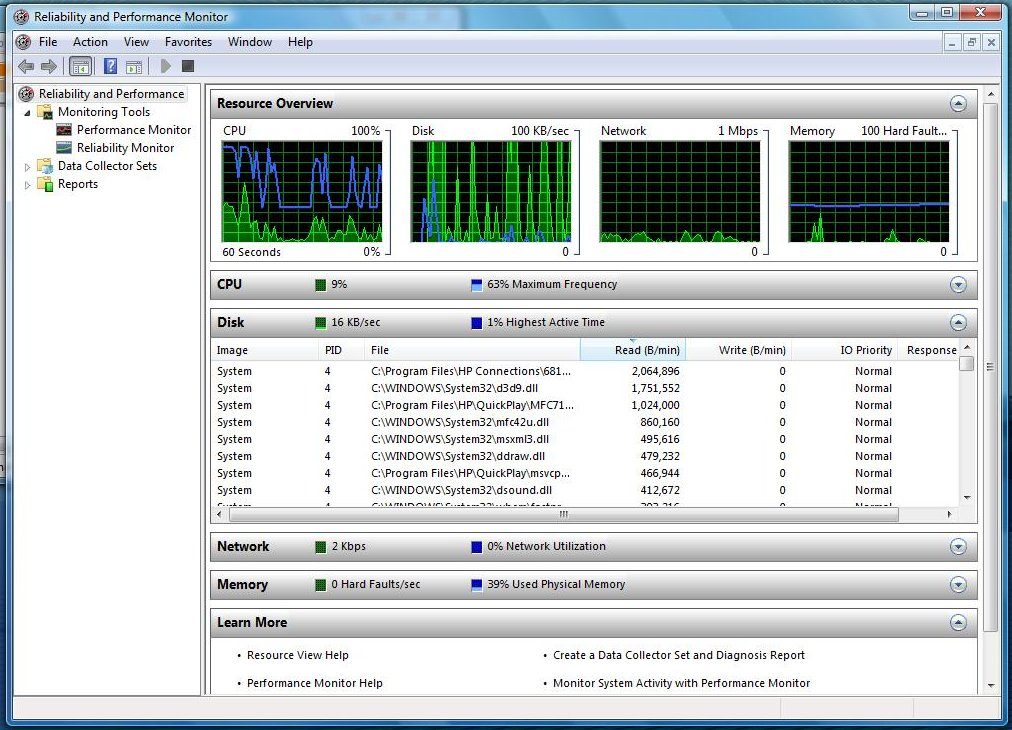
\includegraphics[width=8cm]{images/edl_performance_window.jpg}
        \caption{\label{pic:edl_performance_window}Interface de suivie de performance de Windows.}
        \end{figure}
    
    
    Les données récoltées peuvent être utilisées pour l'évaluation des performances et le réglage. Chaque famille de processeurs possède un jeu différent de compteurs matériels, souvent avec des noms différents, même pour les mêmes types d'événements. Les modèles d'une même famille de processeurs peuvent également différer en fonction des événements spécifiques disponibles. En général, des types d'événements similaires sont disponibles sur la plupart des CPU.

    Malheureusement l'adoption à grande échelle des compteurs matériels a été ralentie par le manque de documentation et le manque d'interfaces multi-plateformes. Historiquement, les compteurs matériels étaient utilisés en interne par les concepteurs de puces et les interfaces n'étaient pas toujours documentées ou mises à la disposition du public. Pour ces raisons, nous estimons qu'il est important de présenter les compteurs et les moyens les plus efficaces de les utiliser. Aujourd'hui encore, ce domaine souffre d'un manque de documentation et d'exemples qui sont deux raisons pour expliquer le manque d'outils que nous regrettons est qui est une des principales motivations de ce travail de thèse. D'autres freins ont rendu le développement des outils de profilage difficile comme le manque d'interface unique pour les différentes plateformes ou la nécessité d'avoir des droits privilégiés (noyau) pour accéder aux compteurs. 
    
    

    \subsubsection{Les registres}
    %%%%%%%%%%%%%%%%%%%%%%%%%%%%%%%%%%
    
        Pour pouvoir suivre l'activité d'un processeur lors de son fonctionnement, les architectures se sont dotées de matériels spécifiques appelés compteurs matériels (\textit{hardware counter}). À l'origine, ce dispositif était utilisé seulement par le constructeur des puces à des fins de débogage lors de leur conception. Avec le processeur 80386, Intel a introduit deux registres matériels, TR6 et TR7, pour réaliser des tests sur le Translation Look-aside Buffer (TLB). Intel précisa alors que ces deux registres ne seraient présents que sur cette version du processeur. Cependant Intel conserva ces deux registres et en ajouta trois dans la version suivante du processeur, le 80486, tout en répétant que ces registres pouvaient disparaître d'une version à l'autre. Cependant, les utilisateurs se sont approprié ces compteurs pour programmer leurs propres outils d'analyse de performance. Ces outils ne fonctionnaient alors plus après qu'Intel ait retiré ces compteurs dans la version suivante (Intel 80586). Cependant, avec l'arrivé du Pentium, Intel à fournit aux développeurs un moyen, expérimental, et lui aussi temporaire, d'accéder de manière uniforme aux différents compteurs: les Model Specific Registers ou MSR.

        Les registres sont séparés en deux familles: les registres architecturaux et non architecturaux. 
        La première famille regroupe les \textbf{registres architecturaux} qui ne "\textit{devraient}"\footnote{Documentation Intel - \textit{The MSRs in the Pentium processor are not guaranteed to be duplicated or provided in the next generation IA-32 processors}} pas disparaître d'une version à l'autre d'un processeur. Pour des raisons historiques, ces registres sont référencés depuis le Pentium 4 avec le prefix \verb|IA32_|. En plus de ne pas disparaître avec les nouvelles architectures, ces registres ne varient pas non plus entre différentes lignes de produit et peuvent aussi être utilisés sur un processeur de téléphone comme sur un processeur de serveur. Par exemple, le registre \verb|IA32_TIME_STAMP_COUNTER| est localisé à l'adresse \verb|0x10| depuis le processeur Pentium. Ce compteur est incrémenté à chaque cycle d'horloge (de base). La fréquence d'incrémentation de ce registre ne varie pas avec celle du processeur et permet de mesurer très précisément un intervalle de temps entre deux mesures. 
        Les registres \textbf{non architecturaux}, quant à eux ne sont pas assurées d'être présent sur de futures architectures. Par exemple, le registre utilisé pour mesurer le nombre de calculs flottants réalisés par un coeur a été retiré entre les architectures Sandy Bridge et Haswell avant de réapparaître ensuite. 
    
    
    \subsubsection{Évènements}
    %%%%%%%%%%%%%%%%%%%%%%%%%%%%%%%%%%
    
        Qu'ils soient architecturaux ou non, le but des MSR est de permettre à l'utilisateur de mesurer le nombre d'occurrences d'un évènement. Cet évènement peut être matériel (cycle d'horloge, exécution d'une instruction, manque dans un cache...) ou logiciel (faute de page, changement de contexte...). Comme les évènements dépendent de la présence ou non des compteurs correspondants, la pérennité des évènements n'est pas assurée d'une architecture à l'autre. Lors du développement d'un outil d'analyse de performance, il est nécessaire de vérifier qu'ils sont disponibles avec l'architecture utilisée. Intel propose la liste des évènements compatible avec chaque architecture \footnote{Liste des évènements compatibles par architecture Intel - \url{https://download.01.org/perfmon/index/}}.
            
        
    
    \subsubsection{Les PMU}
    %%%%%%%%%%%%%%%%%%%%%%%%%%%%%%%%%%
    
        Les évènements peuvent être collectés à différents endroits du processeur grâce à un matériel dédié appelé PMU (\textit{Performance Monitoring Unit}). Leur séparation du reste du processeur permet de ne pas impacter la performance de ce dernier, rendant la collecte d'informations non intrusive. Les PMU sont disposées à différents endroit du processeur: certaines sont rattachées à un coeur spécifique, d'autres sur le processeur lui même (voir \autoref{pic:yamb_skl_pmu}).  Une architecture comme celle des processeurs Skylake possède une PMU par coeur logique et une PMU \textit{uncore}.  Pour pouvoir compter des évènements, la PMU doit être configurée à l'aide de registres matériels MSR.
        
        \begin{figure}[h!]
        \center
        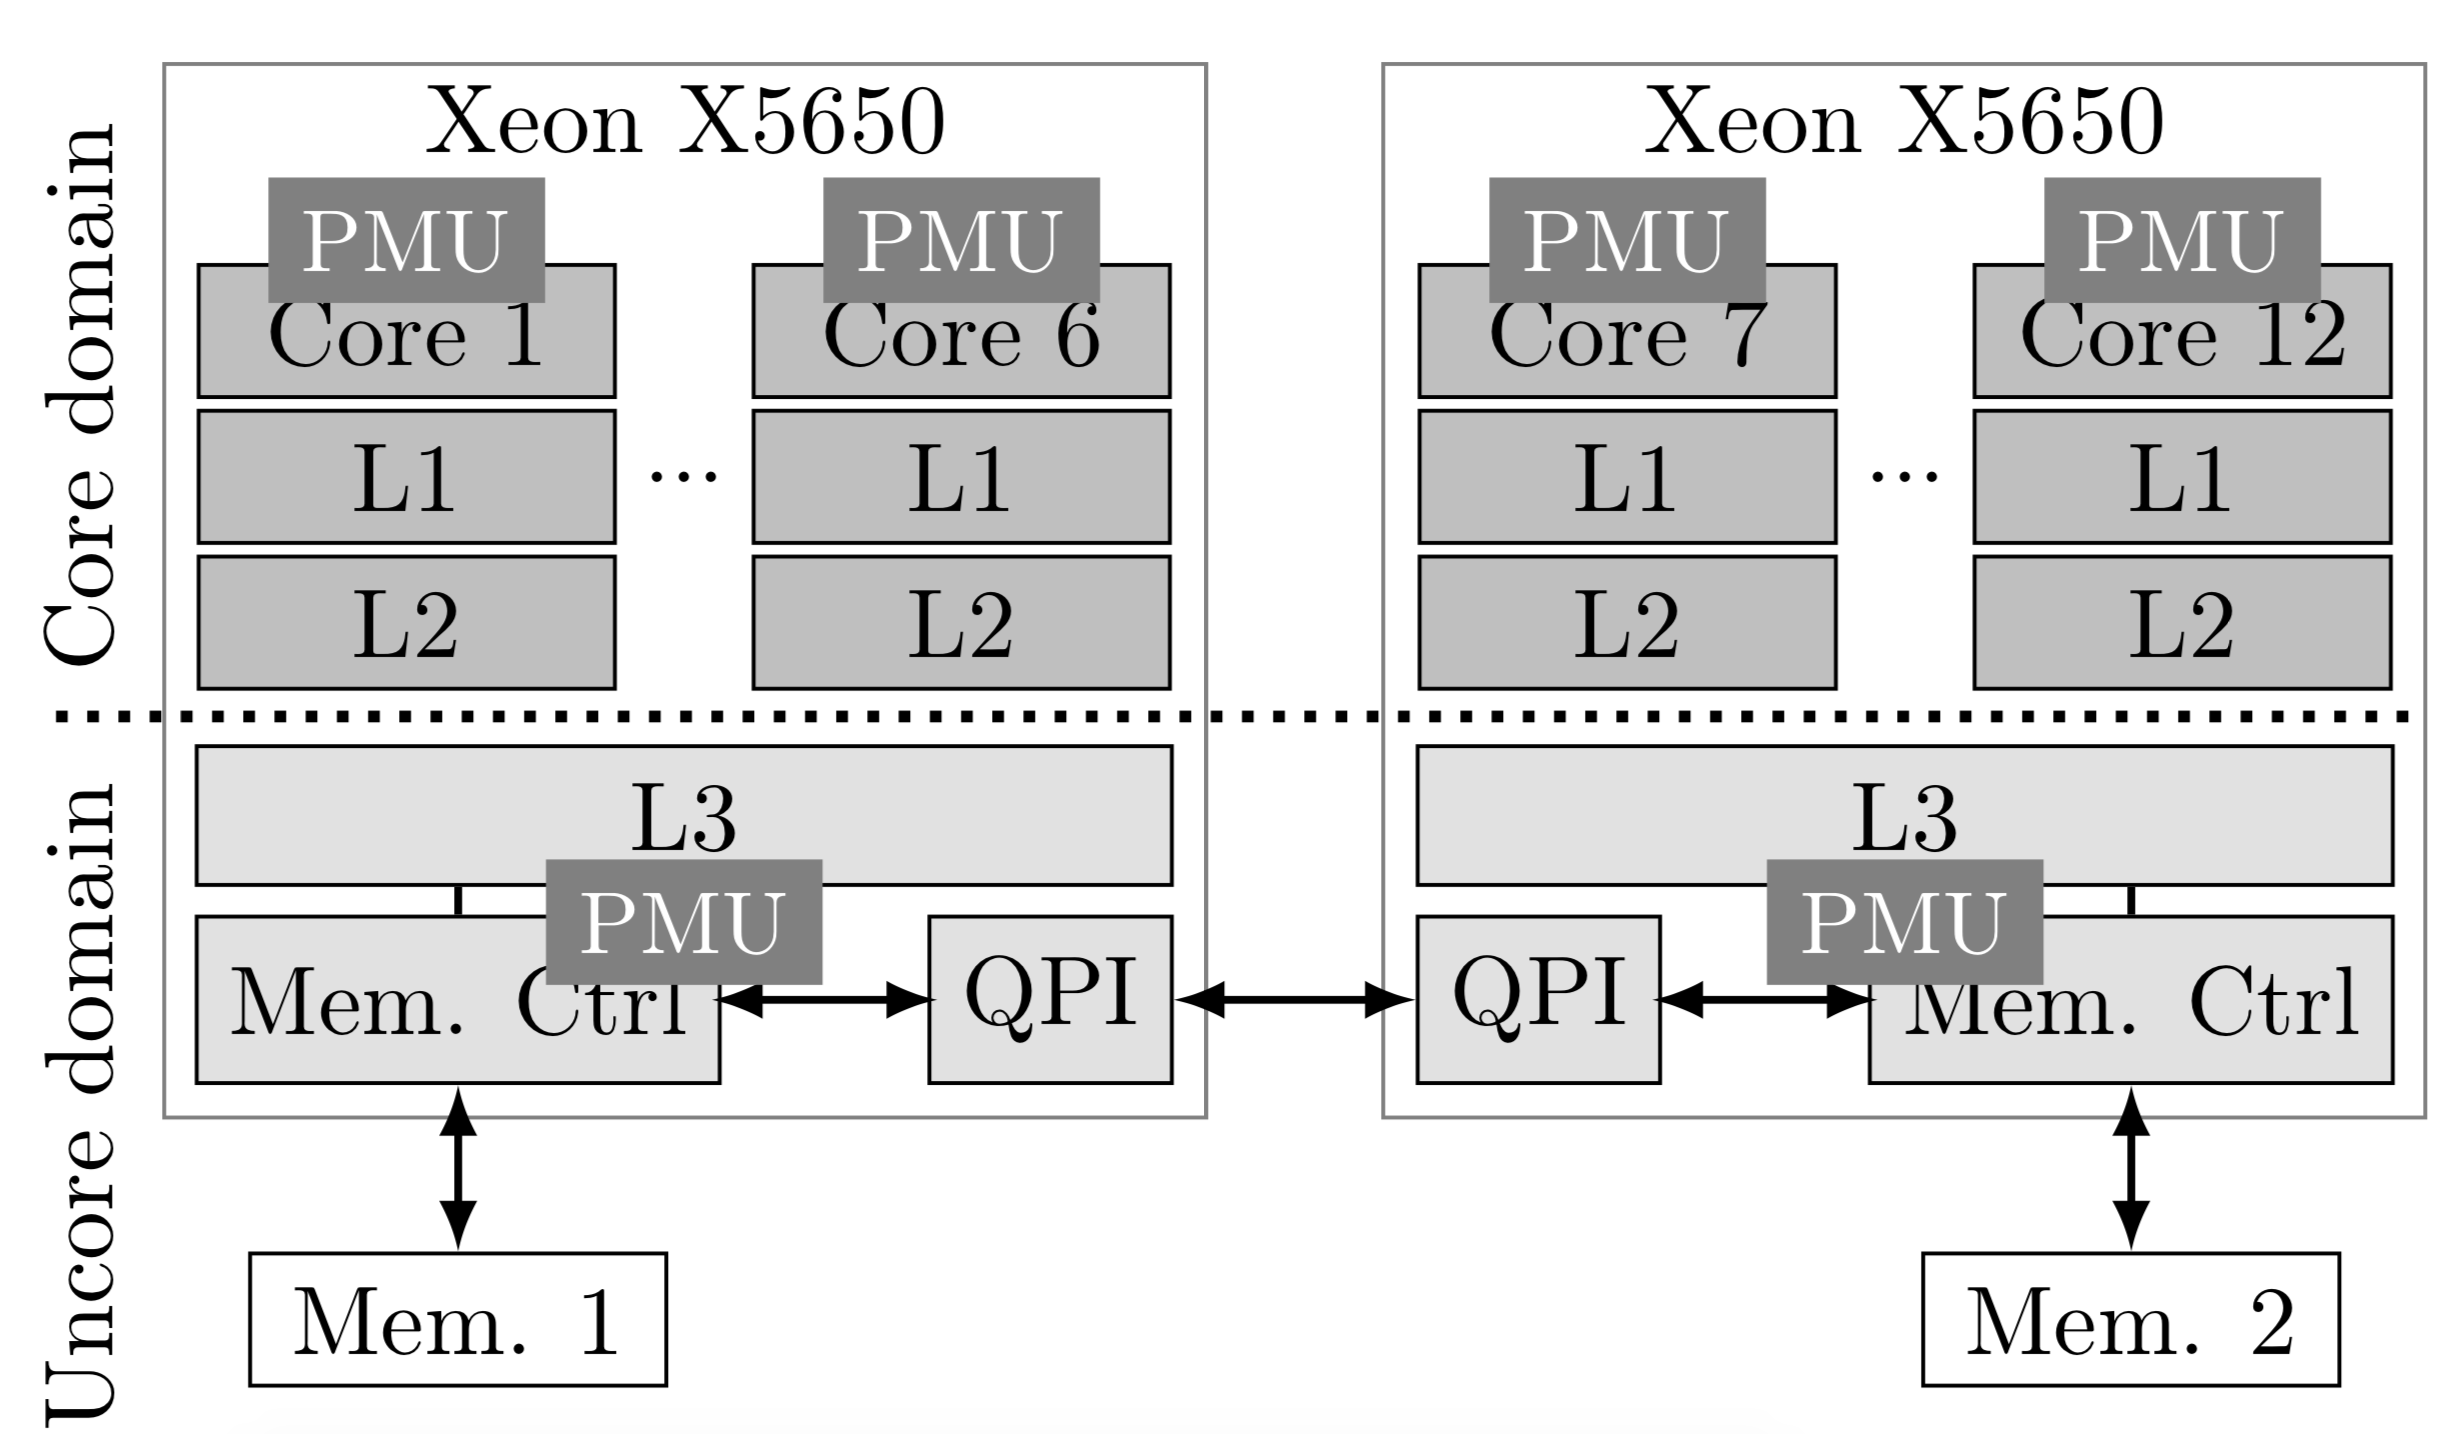
\includegraphics[width=10cm]{images/yamb_skl_pmu.png}
        \caption{\label{pic:yamb_skl_pmu}Exemple de disposition des PMU sur un processeur Skylake (extrait de \cite{Selva2017})}
        \end{figure}
        
        Les mesures réalisées par la PMU peuvent être filtrées pour mesurer la totalité de l'activité ou seulement celle d'un processus. Ces configurations sont réalisées  directement depuis le code (compilateur, manuellement) ou depuis le système (outils de profilage, noyau). Les PMU peuvent être utilisées de deux façons différentes pour étudier l'activité d'un processeur: le comptage et l'échantillonnage. 
        
        \paragraph{Le comptage.} La première méthode consiste à compter le nombre d'évènements arrivant entre deux intervalles de temps. Pour cela, le compteur est initialisé à $0$ et lu au bout d'une certaine période de temps. Les valeurs ainsi récupérées permettent de mesurer le nombre d'occurrences de ces évènements. Cette méthode est efficace, mais elle ne permet pas de connaître la partie du code responsable d'un évènement. Les ratios d'évènements, tels que les instructions exécutées par cycle, les taux de \textit{miss} de mémoire cache et les taux d'erreurs de prévision des branches, peuvent être calculés en divisant le nombre par le temps écoulé.
        
        \paragraph{L'échantillonnage.} Pour obtenir plus d'informations sur le code responsable des évènements, le mode d'échantillonage ou \textit{sampling} doit être utilisé. Ce mode consiste à déclencher une interruption tous les $n$ évènements et sauvegarder certaines informations telles que le pointeur d'instruction. Pour cela, le registre de comptage est initialisé à la valeur $\text{MAX} - n$ ou $\text{MAX}$ correspond à la valeur maximale pouvant être stocké dans le registre. Lorsque $n$ évènements sont comptés, le registre déclenche un débordement (\textit{overflow}) et génère une exception traitée par le système d'exploitation. Grâce à un échantillonage assez fin (nombre $n$ petit) et des méthodes de statistiques, il est possible d'approcher le nombre d'évènements généré par chaque instruction. La principale difficulté de cette technique est d'assurer suffisamment de précision lors de l'attribution d'un évènement à une instruction. En effet, entre le moment où l'interruption est générée et son traitement, plusieurs instructions peuvent avoir été exécutées. Des technologies telles que Intel PEBS\footnote{Documentation Intel - Intel 64 and IA-32 Architectures Software Developer's Manual Volume 3B, Chapter 18. \url{https://software.intel.com/sites/default/files/managed/7c/f1/253669-sdm-vol-3b.pdf}} (Processor Event-Based Sampling) ou AMD IBS (Instruction Based Sampling) \cite{Drongowski2007} agrémentent le processeur d'un tampon lui permettant de stocker les informations nécessaires. L'autre avantage de cette technologie est de réduire l'impact sur les performances dû au traitement de chaque échantillon par le système d'exploitation. La PMU possède un tampon pouvant stocker plusieurs échantillons et n'interrompt l'exécution que lorsque ce tampon est plein. Le principal désavantage de cette technologie est le nombre restreint d'évènements compatibles. De plus, elle n'est pas compatible avec toutes les architectures réduisant la portabilité des outils l'utilisant.
   
        \paragraph{Le multiplexage.}
        Le nombre de registres MSR pouvant être utilisé pour compter un évènement est bien inférieur au nombre d'évènements supportés par l'architecture impliquant de réaliser un choix des évènements à mesurer. De plus, certains évènements ne peuvent pas être mesurés en même temps pour des raisons architecturales. 
        Pour cela, on a recours à des techniques de multiplexage dont le principe est d'exécuter plusieurs groupes de compteurs matériels en suivant un algorithme d'ordonnancement de type \textit{round-robin.} Pour ce faire, un premier groupe d'évènements est mesuré pendant un court intervalle de temps, puis les évènements sont remplacés par ceux du groupe suivant. Ce remplacement est réalisé jusqu'à ce que le comptage d'évènements soit finalement arrêté. Le multiplexage signifie qu'aucun des groupes de compteurs n'a été exécuté sur l'ensemble du code et que l'on ignore quelle fraction du code a été mesurée avec quel groupe. On suppose que la charge de travail est suffisamment uniforme pour que le nombre d'évènements mesurés puisse être étalonné comme si les groupes avaient été exécutés séparément sur le code entier. 
        Les techniques de reconstruction des profils peuvent être inexactes\cite{Lim}. De la même façon que pour l'échantillonnage, l'erreur d'estimation augmente avec le nombre d'évènements à mesurer impliquant un partage plus long des PMU. Pour pouvoir utiliser le maximum de compteurs, il est important de noter que la désactivation de l'\textit{hyperthreading} sur les processeurs Intel, désactive aussi la moitié des compteurs disponibles (voir \autoref{pic:edl_perf_pmu}).



    \subsubsection{Compteurs matériels des architectures Intel}
    %%%%%%%%%%%%%%%%%%%%%%%%%%%%%%%%%%
        

        Pour compter le nombre d'occurrences d'un évènement, les PMU des processeurs Intel possèdent deux types de compteurs: les \textit{Fixed-function counters} (FFC) et les compteurs de performance (HPMC). Les processeurs Intel possèdent une PMU \textit{uncore} directement sur le processeur et une PMU par coeur logique, donc deux PMU par coeur physique lorsque l'\textit{hyperthreading} est activé (voir \autoref{pic:edl_perf_pmu}). Chaque PMU \textit{oncore} possède 3 compteurs \textit{Fixed-Function} et 4 compteurs HPMC.
        
        \begin{figure}
        \center
        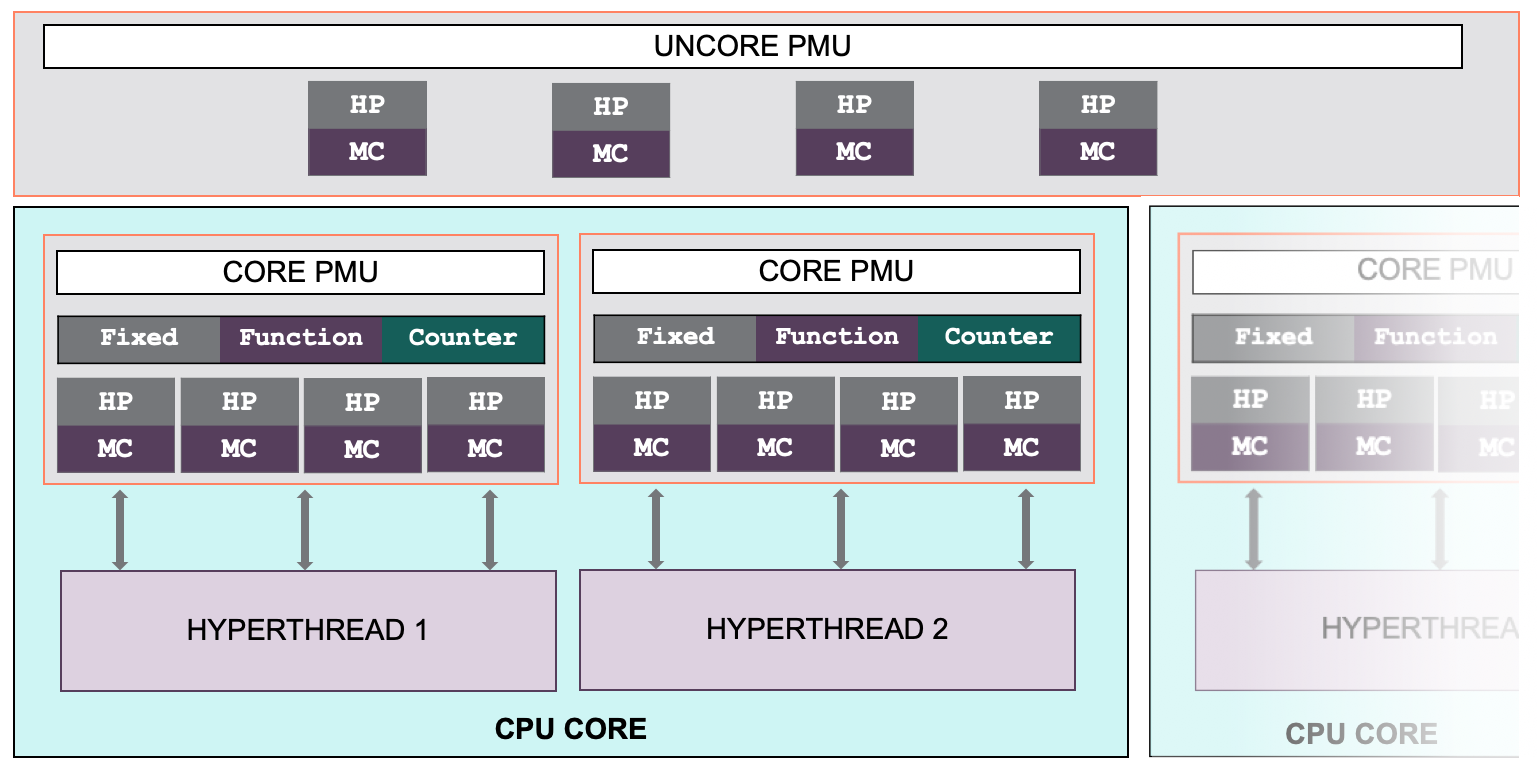
\includegraphics[width=12cm]{images/edl_perf_pmu.png}
        \caption{\label{pic:edl_perf_pmu} Disposition des compteurs matériels sur un coeur d'un processeur Intel.}
        \end{figure}
    
        %%%%%%%%%%%%%%%%%%%%%%%%%%%%%%%%%%%%%%%%%%%%%%%%%%%%%%%%%%
        \paragraph{Les compteurs FFC}
        Les compteurs \textit{Fixed-Function} sont les plus simples à utiliser, car ils sont déjà configurés pour compter un évènement. Sur les architectures Intel, il y a 3 compteurs FFC par coeur logique. Le premier compteur (\textit{IA32\_FIXED\_CTR0}) compte le nombre d'instructions exécutées par un coeur. Le deuxième (\textit{IA32\_FIXED\_CTR1}), compte le nombre de cycles à la fréquence nominale du processeur. Enfin le troisième (\textit{IA32\_FIXED\_CTR3}), compte le nombre de cycles durant lequel le coeur est actif. Pour pouvoir utiliser ces trois compteurs, une simple configuration est requise grâce aux deux registres \textit{IA\_32\_PERF\_GLOBAL\_CTRL} et \textit{IA\_ Le 32\_FIXED\_CTR\_CTRL} (voir \autoref{pic:edl_perf_ffc}). 
        
        \begin{figure}[h!]
        \center
        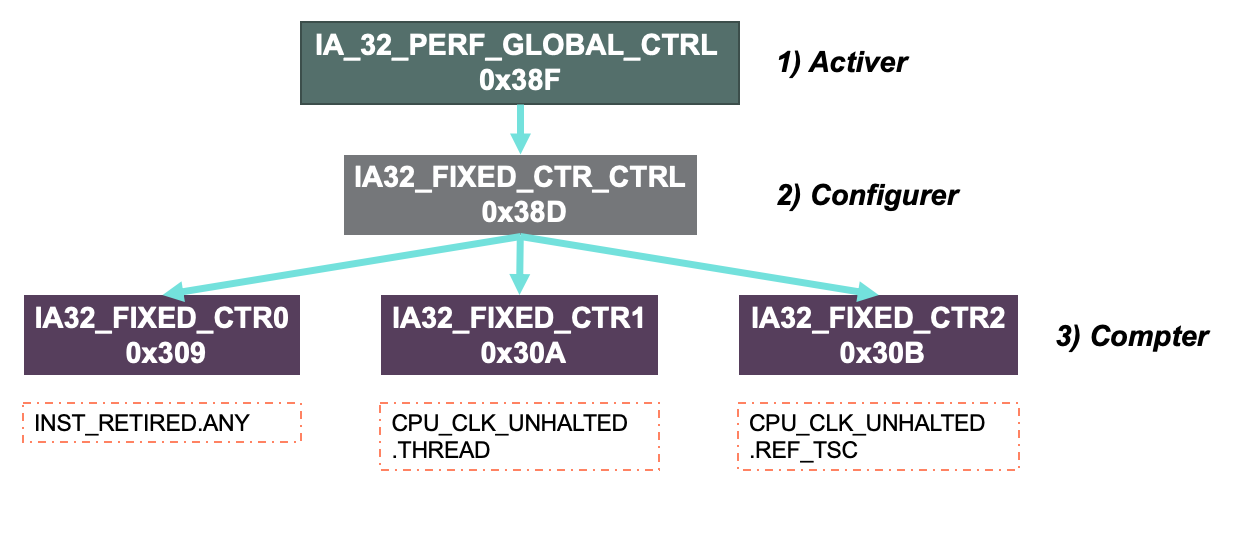
\includegraphics[width=10cm]{images/edl_perf_ffc.png}
        \caption{\label{pic:edl_perf_ffc} Chaque coeur logique dispose d'une PMU possédant 3 compteurs pré-configurés pour compter un type d'évènement.}
        \end{figure}
        
        Le premier MSR permet d'activer les deux types de compteurs (HPMC et PPF). Chaque bit de ce registre correspond à l'activation ou non du compteur associé. Cette activation n'a à être réalisée qu'une seule fois au démarrage du processeur. Le deuxième registre permet de configurer le comptage d'événements: mode utilisateur ou noyau, mesure du coeur logique associé ou de tout le coeur physique, ainsi que de permettre au compteur de générer ou non une interruption lorsque celle-ci dépasse la valeur maximale pouvant être stockée sur 48 bits. Ce dernier bit de configuration peut être utilisé pour vérifier l'utilisation ou non du compteur par un autre programme (qui voudrait être alerté par une interruption). Une fois ces deux opérations réalisées (activation et configuration), les évènements sont comptés dans les trois registres correspondants, il ne suffit alors plus que de lire la valeur s'y trouvant. Bien qu'il ne soit pas nombreux, les trois compteurs FFC permettent d'obtenir des informations intéressantes sur l'utilisation du processeur. Par exemple en divisant le troisième compteur par le deuxième ($\frac{IA32\_FIXED\_CTR3}{IA32\_FIXED\_CTR2}$) on obtient le pourcentage d'utilisation du coeur. En utilisant le premier compteur, on peut aussi obtenir un bon indicateur sur la performance du code: le nombre d'instructions exécutées chaque cycle (IPC).
        
       
        
        
        %%%%%%%%%%%%%%%%%%%%%%%%%%%%%%%%%%%%%%%%%%%%%%%%%%%%%%%%%%%%%%%%%%%
        \paragraph{Les compteurs HPMC.} Les compteurs HPMC sont plus difficiles à utiliser, ils doivent être configurés par l'utilisateur et la longue documentation (plusieurs centaines de pages) n'est pas toujours évidente à comprendre. Les compteurs HPMC sont présents sur les PMU des \textit{oncore} et \textit{uncore}. Leur nombre dépend de l'architecture, les derniers processeurs Skylake possèdent 4 compteurs HPMC par PMU \textit{oncore}, donc 8 compteurs par coeur. Un compteur HPMC est composé de deux registres. L'un est utilisé pour la configuration, le deuxième pour le comptage (voir \autoref{pic:edl_perf_hpmc}).
        
       \begin{figure}[h!]
        \center
        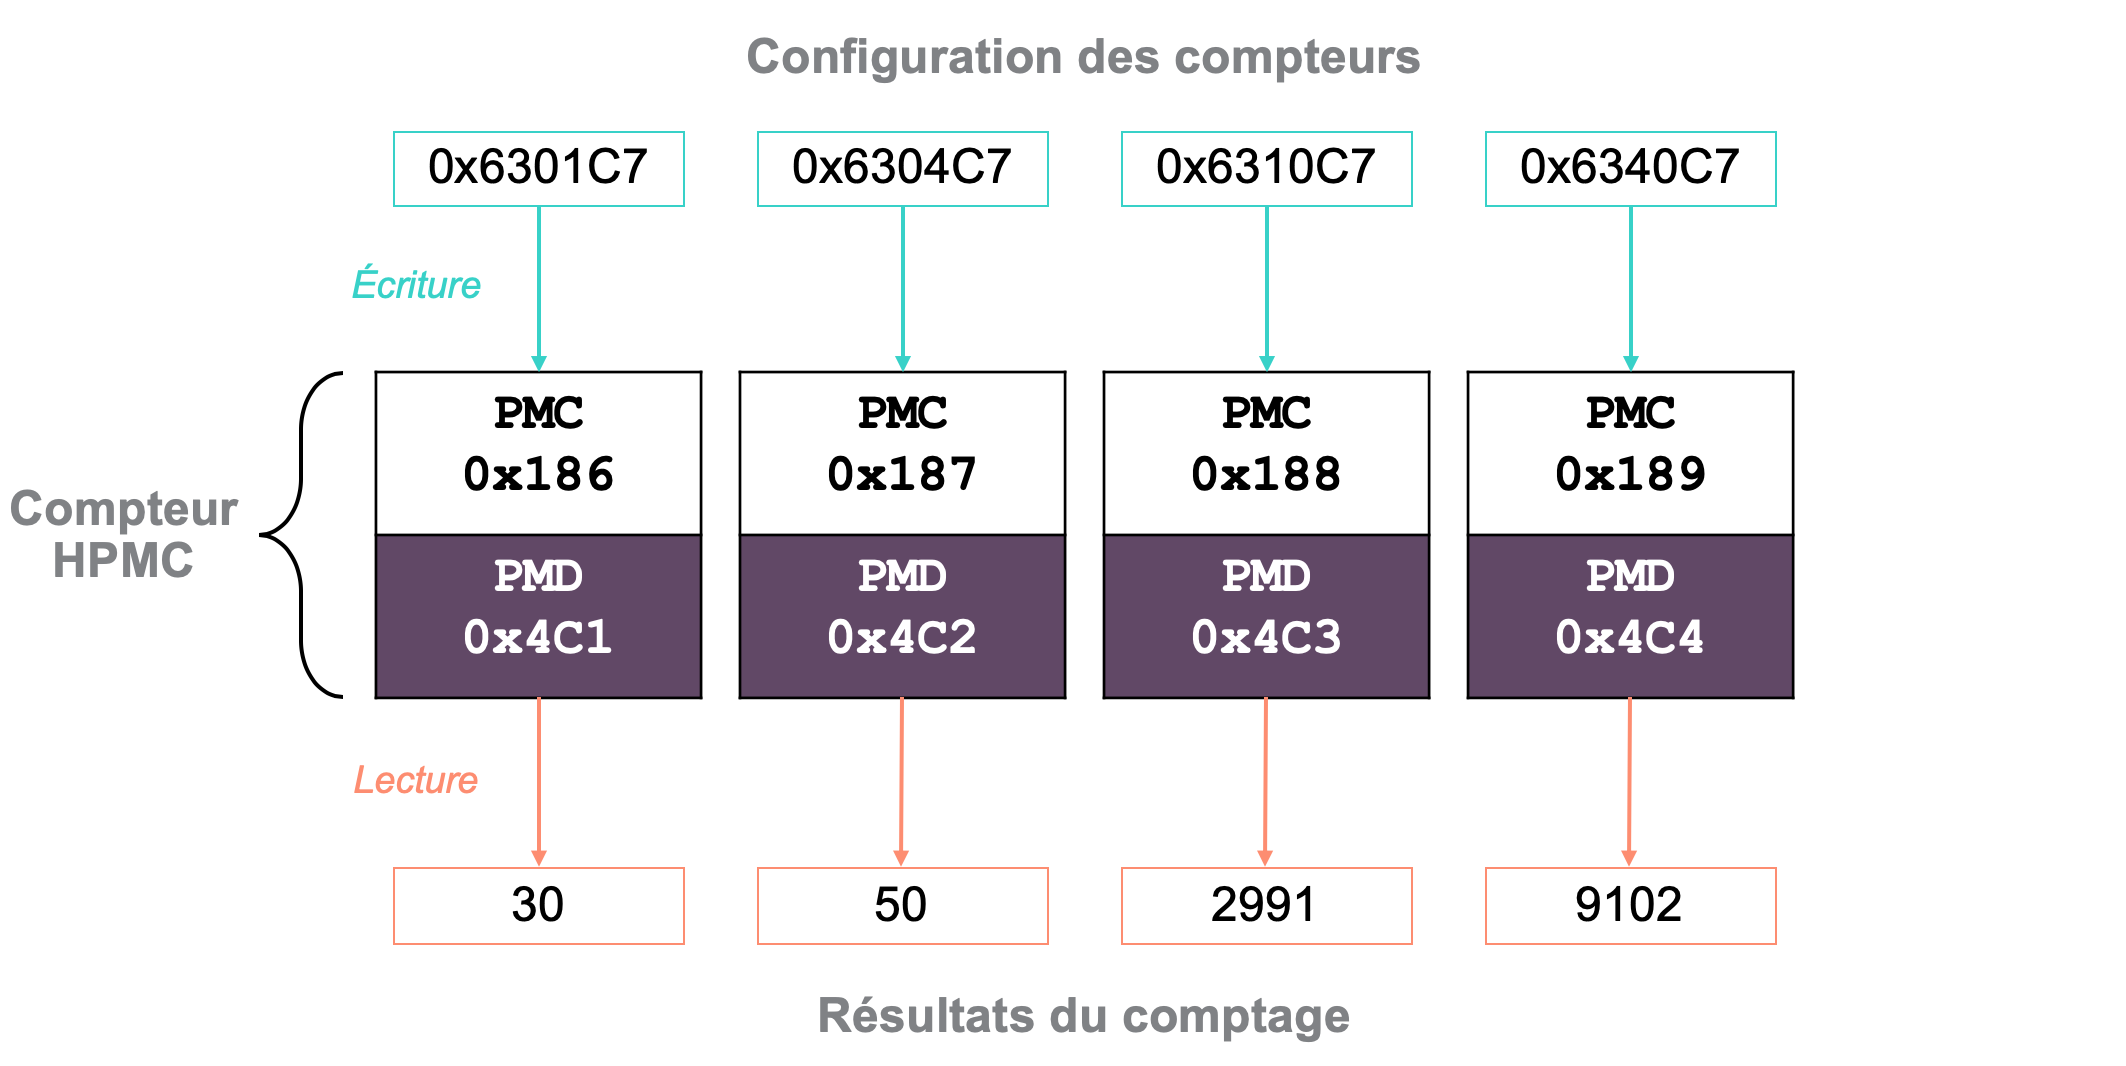
\includegraphics[width=14cm]{images/edl_perf_hpmc.png}
        \caption{\label{pic:edl_perf_hpmc} Chaque coeur logique dispose d'une PMU possédant 4 compteurs HPMC pouvant être configurés pour compter différents évènements. Dans cet exemple, les 4 compteurs sont configurés pour compter toutes les opérations flottantes en doubles précisions exécutées sur le coeur (opérations scalaires et vectorielles (128, 256 et 512 bits)).}
        \end{figure}
        
        Le premier registre est appelé PMC (Performance Monitoring Controler) référencé sous le nom \verb|IA32_PERFEVTSELx|. Chaque HPMC possède son propre registre PMC (accessibles aux adresses 0x186, 0x187, 0x188 et 0x189) qui permet de réaliser la configuration des quatre compteurs: activation, génération d'une interruption, mode (utilisateur ou noyau), évènement à compter (voir \autoref{pic:eld_perf_pmc}). Le \autoref{tab:pmc_config} montre un exemple de configuration d'un compteur pour compter le nombre instructions flottantes scalaires exécutées. Il faut pour cela trouver le code correspondant dans la documentation Intel \cite{Intel2018} au chapitre 19.2 pour les évènements Skylake. Ensuite, les différents bits de configuration sont utilisés pour activer le compteur et filtrer les évènements à compter (système d'exploitation et/ou utilisateur). La valeur résultante (\verb|0x6301C7|) n'a plus qu'à être écrite dans un des quatre MSR du coeur pour lancer le comptage dans le registre PMD correspondant.
        
        \begin{figure}
        \center
        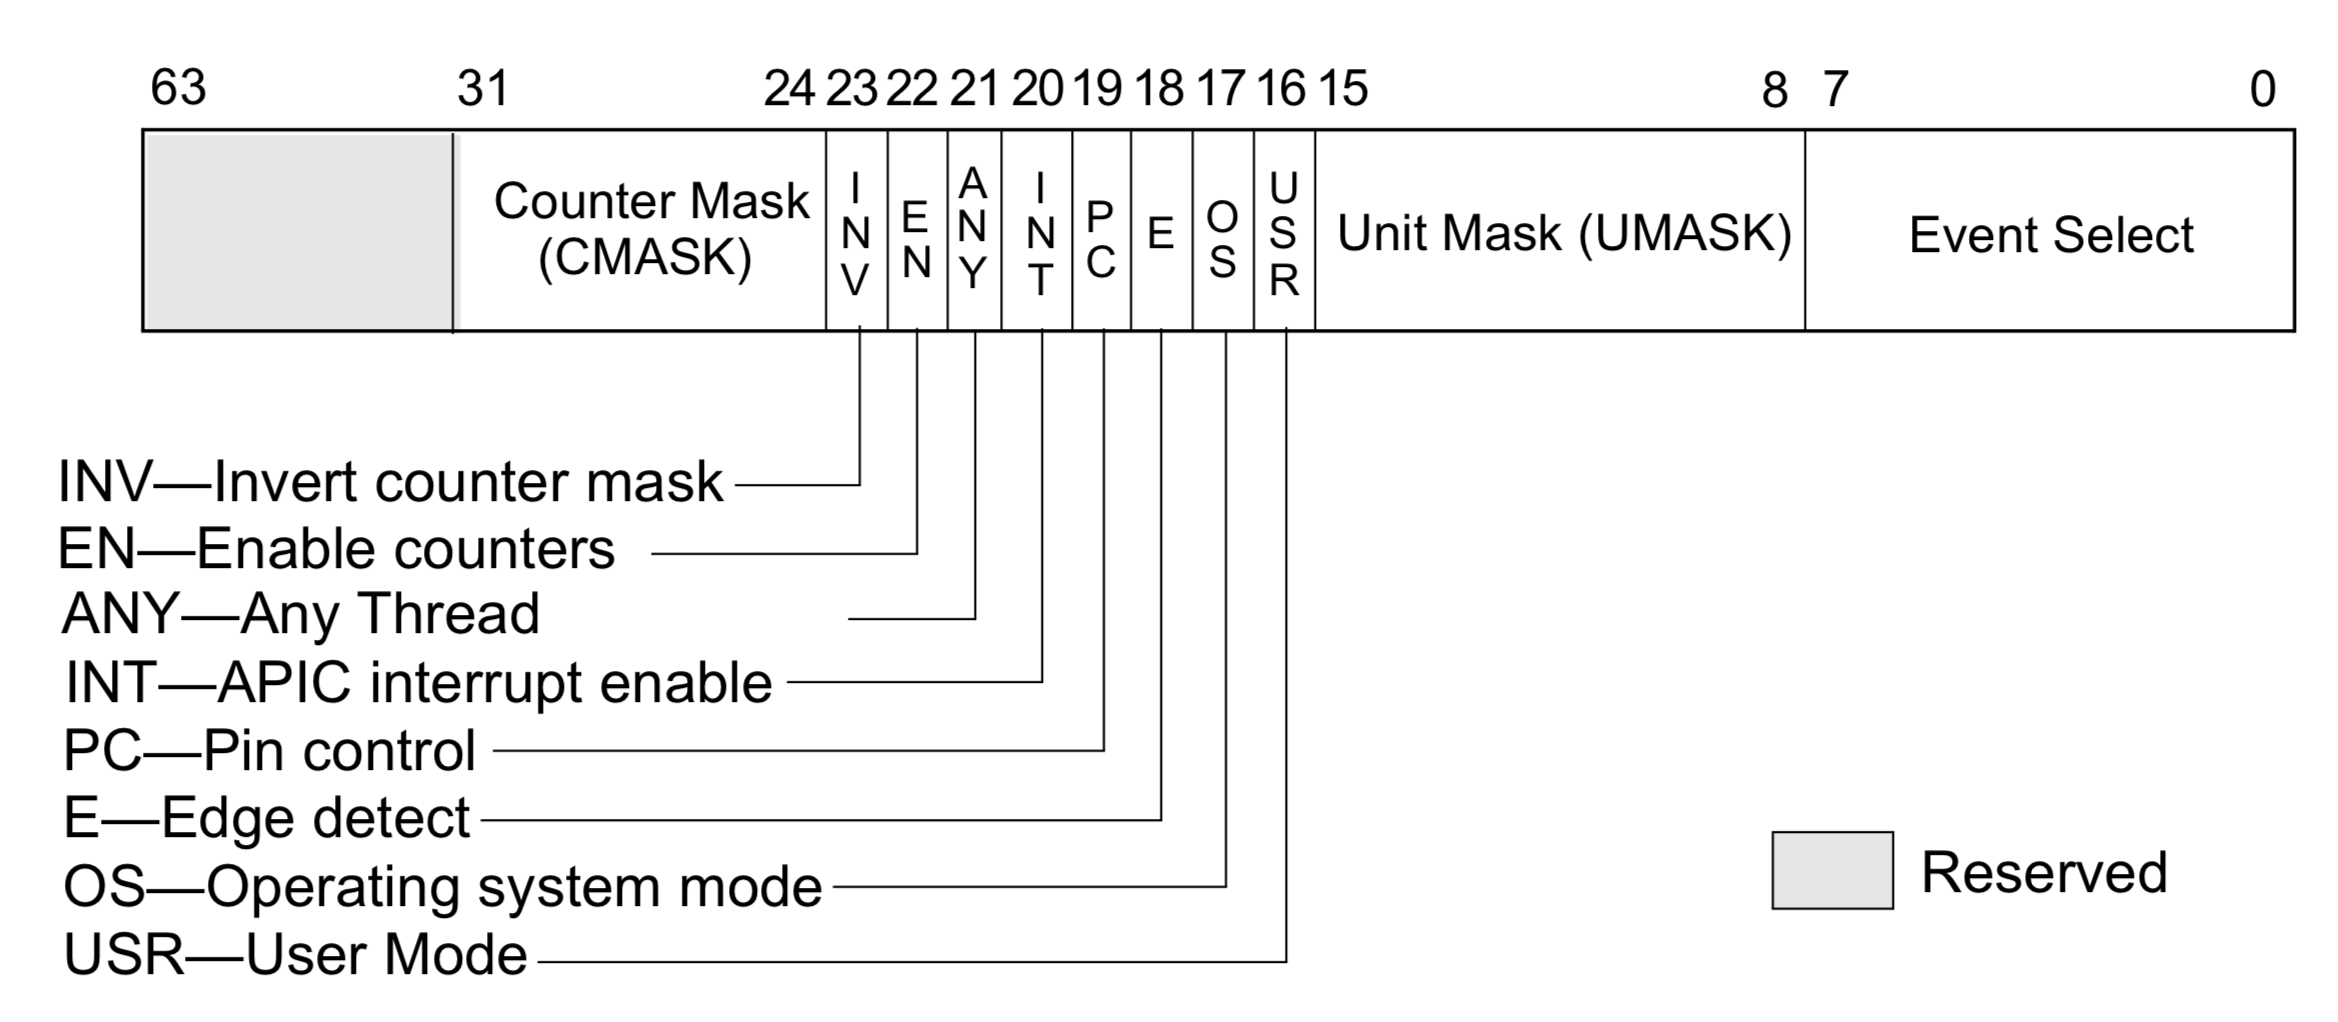
\includegraphics[width=8cm]{images/eld_perf_pmc.png}
        \caption{\label{pic:eld_perf_pmc}Organisation du registre MSR utilisé pour la configuration d'un compteur.}
        \end{figure}
        
        
        Le deuxième registre des compteurs HPMC est appelé PMD (Performance Monitoring Data). Il enregistre le nombre d'évènements depuis son activation réalisée avec registre PMC qui lui est associé. Ces MSR sont des registres architecturaux nommés \verb|IA32_PMC| et localisés des adresses \verb|0x4C1| à \verb|0x4C4|.
       
        
        % Please add the following required packages to your document preamble:
        % \usepackage{graphicx}
        \begin{table}[]
        \centering
        \begin{tabular}{l|c|c|c|c|c|c|c|c|c|c|c|}
        \cline{2-12}
        & \multicolumn{1}{l|}{CMASK} & \multicolumn{1}{l|}{INV} & \multicolumn{1}{l|}{EN} & \multicolumn{1}{l|}{ANY} & \multicolumn{1}{l|}{INT} & \multicolumn{1}{l|}{PC} & \multicolumn{1}{l|}{E} & \multicolumn{1}{l|}{OS} & \multicolumn{1}{l|}{USR} & \multicolumn{1}{l|}{UMASK} & \multicolumn{1}{l|}{EVENT} \\ \hline
        \multicolumn{1}{|l|}{bits} & 31 - 24 & 23 & 22 & 21 & 20 & 19 & 18 & 17 & 16 & 15 - 08 & 7 - 0 \\ \hline
        \multicolumn{1}{|l|}{Valeur} & 0 & 0 & 1 & 1 & 0 & 0 & 0 & 1 & 1 & 1 & C7 \\ \hline
        \multicolumn{1}{|l|}{Résultat} & 0 & \multicolumn{4}{c|}{6} & \multicolumn{4}{c|}{3} & 1 & C7 \\ \hline
        \end{tabular}%
        \caption{Configurer un compteur pour compter le nombre d'instructions flottantes exécutées revient à écrire la valeur $0x6301C7$ dans son registres PMC.}
        \label{tab:pmc_config}
        \end{table}
        
  

        
        
    \subsection{Architecture Intel: PMU core} \label{sec:perf_asm_msr}
    %%%%%%%%%%%%%%%%%%%%%%%%%%%%%%%%%%
    
        Au fil des générations, les architectures ont reçu plusieurs instructions permettant d'interagir avec les registres MSR. Les processeurs Intel possèdent actuellement 5 instructions nécessitant différents privilèges pour les exécuter (voir \autoref{fig:edl_perf_assembly_msr}).
        
        \begin{figure}[h!]
            \center
            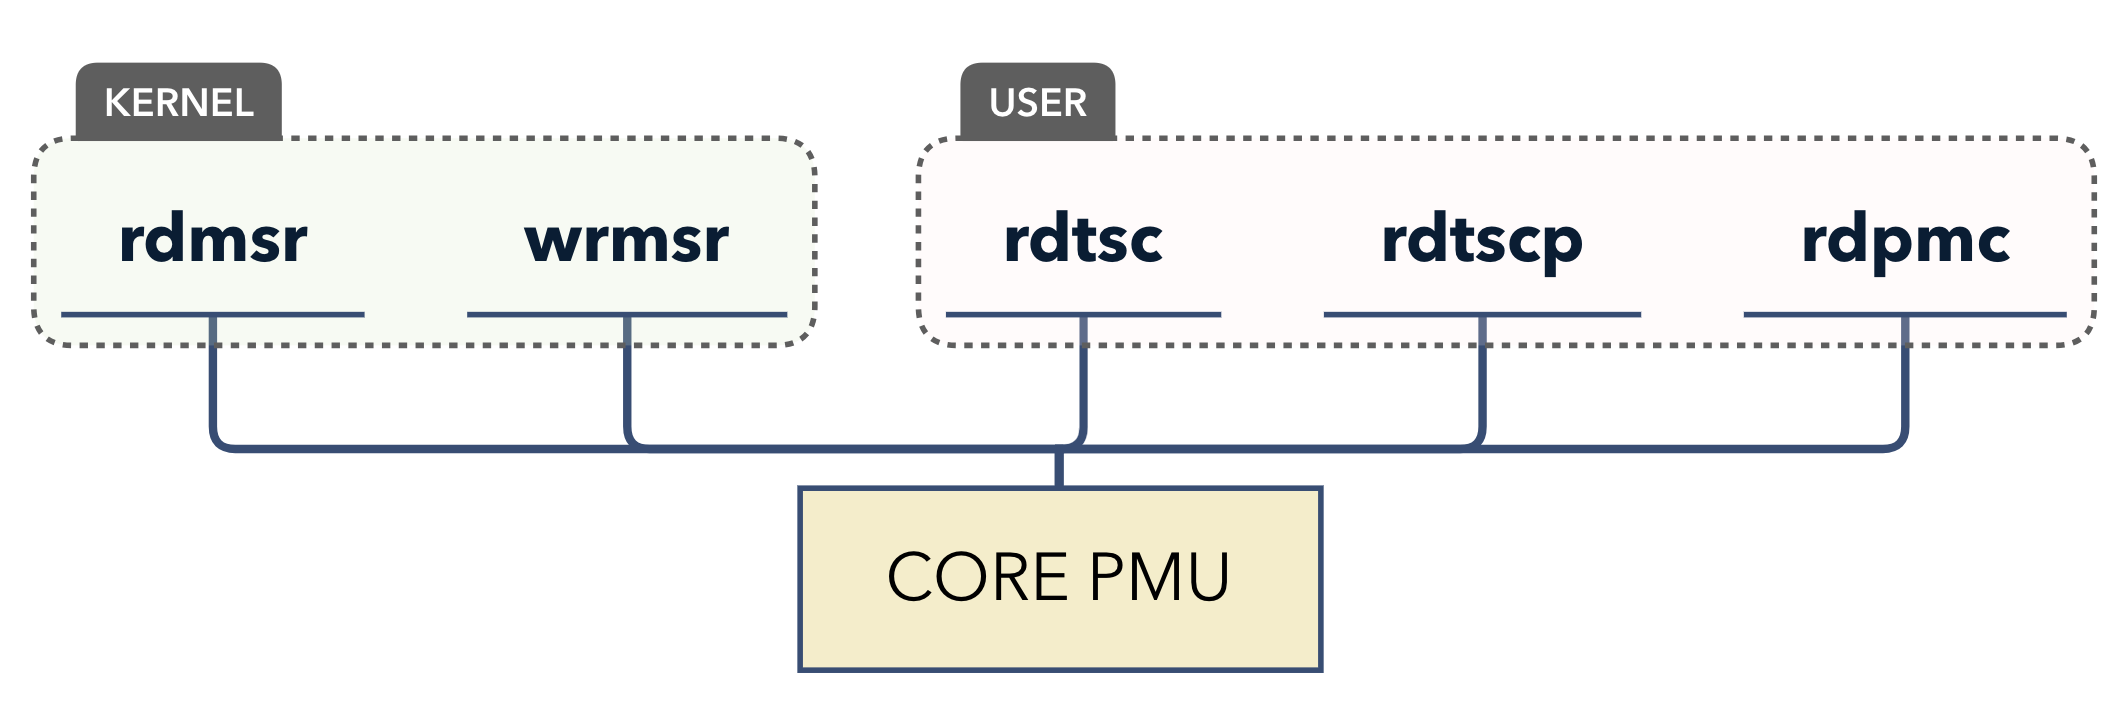
\includegraphics[width=10cm]{images/edl_perf_assembly_msr.png}
            \caption{\label{fig:edl_perf_assembly_msr} Instructions assembleurs permettant d'accéder aux registres MSR d'une architecture Intel.}
        \end{figure}
    
    
        Les compteurs sont des registres matériels, ils peuvent donc être écrits et lus comme n'importe quels autres registres. Il existe deux instructions assembleur permettant d'écrire (\textit{wrmsr}) et de lire (\textit{rdmsr}) ces registres. Les registres accessibles à l'utilisateur peuvent être listés grâce à l'instruction \textit{cpuid}. Cependant, ces instructions ne peuvent être exécutées que par un processus de privilège 0. En effet, laisser la possibilité à un utilisateur normal de modifier ces registres peut être très dangereux pour la sécurité du système. Tous les processus qui veulent interagir avec les registres MSR doivent donc pouvoir accéder à ce niveau de privilège. C'est \textit{la} contrainte majeur qui rend difficile le développement d'outils de suivi de performance. De multiples moyens ont été mis au point depuis pour pouvoir y accéder sans compromettre la sécurité du système. 
        
        Le premier moyen a été introduit par Intel grâce à la création d'une troisième instruction assembleur permettant de lire le contenu d'un registre avec l'instruction \textit{rdpmc}. Cette instruction a ajouté avec la sortie du Pentium Pro en 1995. Bien que cette instruction ne permette par d'écrire dans un registre, elle permet de lire le résultat des compteurs et notamment les compteurs FFC. Ces compteurs étant déjà configurés, l'instruction \textit{rdpmc} permet de pouvoir lire ces trois compteurs sans privilège supplémentaire. Dans un programme C, le compteur \textit{ctr} (1, 2 ou 3) peut être lu grâce au code de l'\autoref{lst:edl_rdpmc_ffc}. L'instruction \textit{rdpmc} peut aussi être utilisé pour lire les compteurs HPMC grâce au code de l'\autoref{lst:edl_rdpmc_pmc}. Cela peut être utile pour laisser les utilisateurs accéder aux résultats des compteurs HPMC après qu'un autre programme ayant les droits d'utilisation de l'instruction \textit{wrmsr} ait paramétré les compteurs.
    
    
    

\begin{minipage}{.45\textwidth}
\begin{lstlisting}[
label=lst:edl_rdpmc_ffc,
basicstyle={\scriptsize\ttfamily},
identifierstyle={\color{black}},
language={c},
tabsize=2,
numbersep=8pt,
frame=tlbr,framesep=2pt,framerule=0pt,
morekeywords ={class,run},
caption=Lecture des compteurs FFC grâce à l'instruction \textit{rdpmc}.
]
ul rdpmc_Fixed-Function (int ctr){
   unsigned a, d, c;
   c = (1<<30) + ctr;
   __asm__ volatile("rdpmc" : "=a" (a), 
                              "=d" (d) 
                            :  "c" (c));
   return ((unsigned long)a) | 
         (((unsigned long)d) << 32);;
}
\end{lstlisting}
\end{minipage}%%
\hfill
%&
%
\begin{minipage}{.45\textwidth}
\begin{lstlisting}[
label=lst:edl_rdpmc_pmc,
basicstyle={\scriptsize\ttfamily},
identifierstyle={\color{black}},
tabsize=2,
language={c},
numbersep=8pt,
xleftmargin=0,frame=tlbr,framesep=2pt,framerule=0pt,
morekeywords ={class,run},
caption=Lecture des compteurs HPMC grâce à l'instruction \textit{rdpmc}.
]
ul rdpmc_counter (int ctr){
   unsigned a, d, c;
   c = ctr;
   __asm__ volatile("rdpmc" : "=a" (a),
                              "=d" (d)
                            :  "c" (c));
   return ((unsigned long)a) | 
         (((unsigned long)d) << 32);;
}
\end{lstlisting}
\end{minipage}




    \subsection{Architecture Intel: PMU uncore}\label{sec:edl_perf_uncore}
%%%%%%%%%%%%%%%%%%%%%%%%%%%%%%%%%%
    
    
    La plus grande partie des CPU modernes se trouve en dehors des coeurs. Sur les processeurs Intel, cette partie est appelée \textit{Uncore} et possède entre autres le lien PCI-Express, le cache de dernier niveau ainsi que les contrôleurs mémoire. Pour suivre les performances de ces matériels, l'\textit{uncore} possède également une PMU permettant entre autres de mesurer la bande passante mémoire ou l'activité du cache LLC. La PMU ne se trouvant pas sur les coeurs directement il est impossible d'associer le déclenchement d'un évènement à un coeur particulier et d'autant moins à un processus. De plus, il n'est pas possible de contrôler les registres MSR directement depuis le coeur grâce aux instructions assembleurs \textit{rdmsr} et \textit{wrmsr} utilisées pour les PMU des coeurs. Cependant, certains des compteurs \textit{uncore} sont dupliqués sur les coeurs et peuvent être accédé de la même manière (\textit{miss} dans le cache LLC par exemple). Pour accéder aux autres compteurs, il est nécessaire de passer par l'interface PCI.
    
     
    \begin{figure}
    \center
    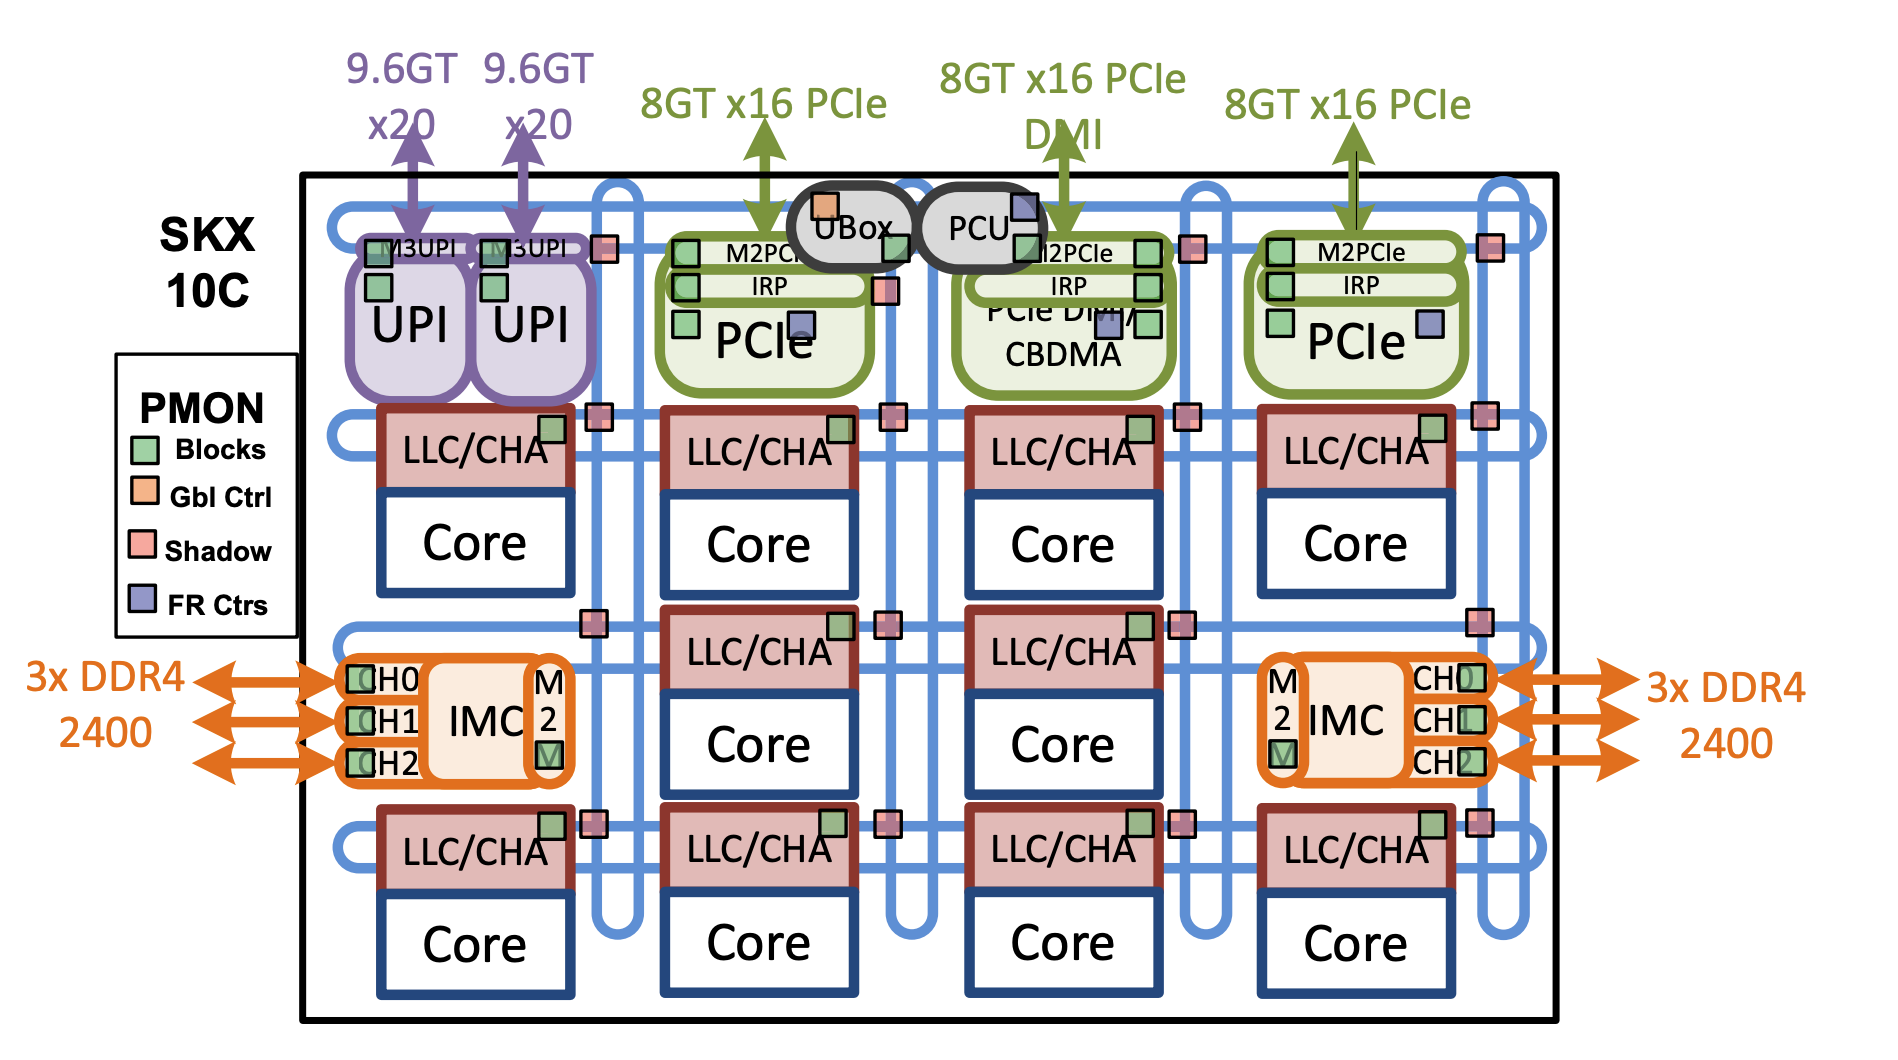
\includegraphics[width=12cm]{images/edl_perf_uncore_intel_skl.png}
    \caption{\label{fig:edl_perf_uncore_intel_skl} Disposition des PMU uncore sur les processeurs Xeon Skylake. \protect\footnotemark}
    \end{figure}
    \footnotetext{source: Intel Xeon Processor Scalable Memory Family Uncore Performance Monitoring Reference Manual.}

    
    \paragraph{Rappel PCI.} 
    Le bus PCI a été défini pour établir un bus local de haute performance et de faible coût. Le composant bus PCI et l'interface de carte d'extension sont indépendants du processeur, ce qui permet une transition efficace vers les futurs processeurs, ainsi qu'une utilisation avec des architectures multiprocesseurs. Pour identifier les différents matériels PCI, la notation BDF est utilisée: \verb| Bus:Device:Function|. Cela permet d'avoir jusqu'à 256 bus, chacun avec jusqu'à 32 appareils, chacun supportant huit fonctions. Chaque fonction de l'appareil sur le bus dispose d'un espace de configuration de 256 octets et impose une structure spécifique. Tous les périphériques compatibles PCI doivent prendre en charge les champs Vendor ID, Device ID, Command and Status, Revision ID, Class Code et Header Type. Par exemple, le matériel construit par le vendeur Intel aura un code 0x8086\footnote{Source: \url{https://pcisig.com/membership/member-companies?combine=Intel}}.
    
    

    \subsubsection{/sys interface}
    %%%%%%%%%%%%%%%%%%%%%%%%%%%%%%%%%%
        L'interface Linux \textit{/sys} est un système de fichier virtuel introduit avec la version 2.6 du noyau Linux. Il permet de présenter les différents \textit{devices} du noyau à l'espace utilisateur. Un \textit{device} peut être un matériel, un driver, un bus... Chaque répertoire représente un matériel, et les fichiers s'y trouvant comportent l'information correspondant à son nom (vendeur, évènement). Les matériels peuvent être représentés par bus, grâce au chemin \verb|/sys/bus| comme présenté dans la \autoref{fig:edl_perf_sys_pci}. Pour accéder aux PMU \textit{uncore}, le driver doit être activé. Il est possible de le vérifier en regardant si plusieurs fichiers nommés \textit{uncore*} apparaissent dans le dossier \verb|/sys/devices/|. Il est ensuite possible de programmer les PMU grâce à des lectures/écritures dans le fichier \textit{config} correspondant au bon matériel. L'exemple suivant permet d'activer les compteurs \textit{FFC}:
   
    
\begin{lstlisting}[
basicstyle={\scriptsize\ttfamily},
identifierstyle={\color{black}},
language={c},
tabsize=2,
numbersep=8pt,
frame=tlbr,framesep=2pt,framerule=0pt,
morekeywords ={class,run},
]
pci_fd = open("/sys/devices/pci0000:3a/0000:3a:0a.6/config",O_RDWR);
ctl = 0x10100UL; // enable + freeze
pwrite (pci_fd, &ctl, sizeof(ctl), BOX_CTL);
\end{lstlisting}

    
    \begin{figure}
    \center
    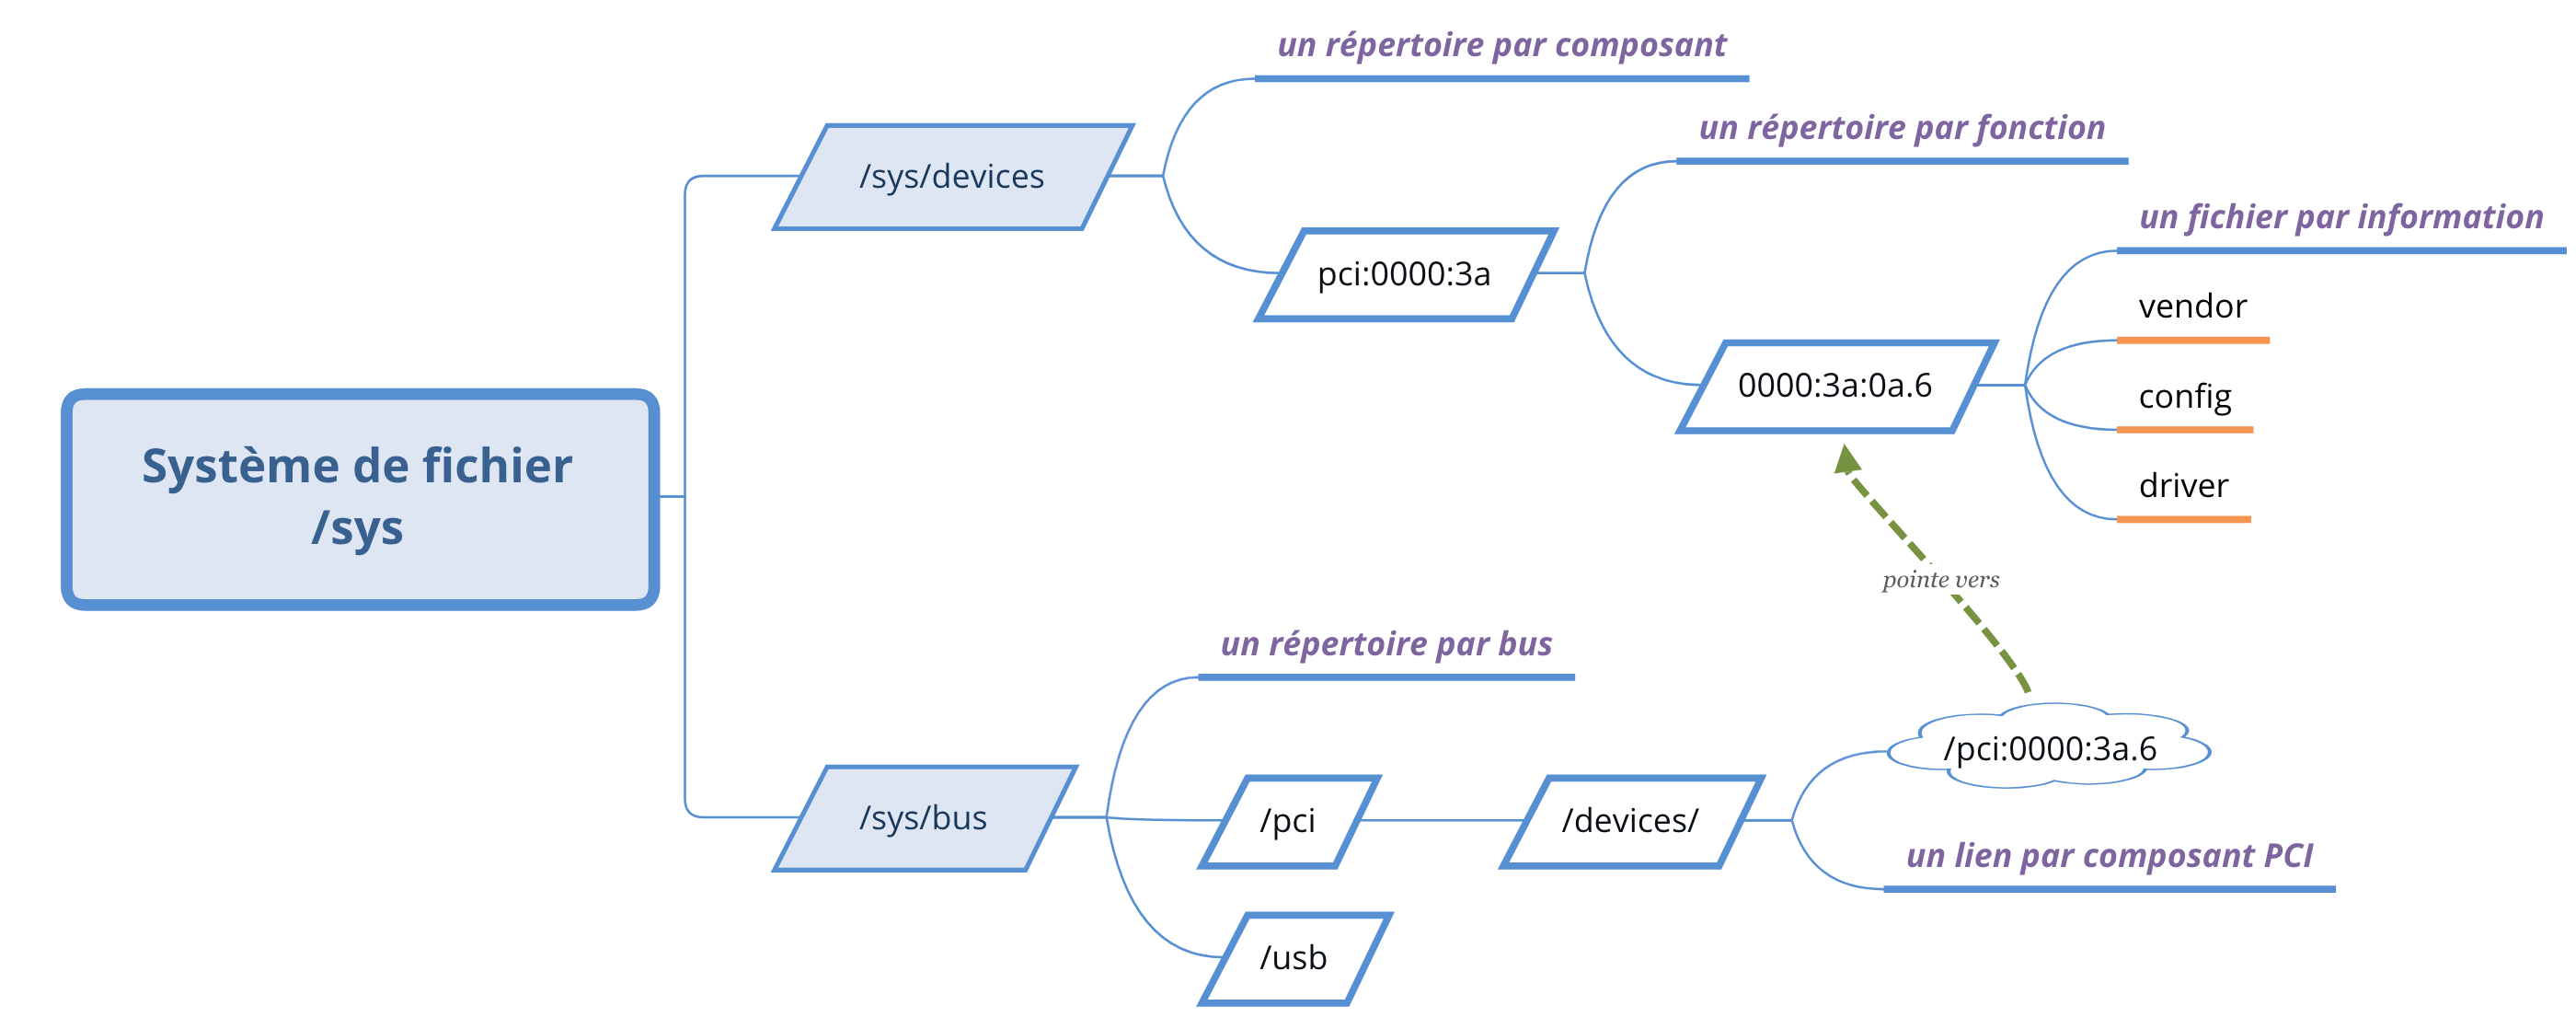
\includegraphics[width=14cm]{images/edl_perf_sys_pci.png}
    \caption{\label{fig:edl_perf_sys_pci} Système de fichier virtuel présentant les matériels PCI.}
    \end{figure}

    
    \subsubsection{lspci + setpci}
    %%%%%%%%%%%%%%%%%%%%%%%%%%%%%%%%%%
    
    Pour interagir avec le matériel PCI, Linux propose deux commandes: \verb|lspci| pour les lister et \verb|setpci| pour les configurer. Cette section présente un exemple de configuration des compteurs permettant de suivre le trafic du bus mémoire d'une architecture Skylake. 
    
    
    
    Comme le montre la \autoref{fig:edl_perf_sys_pci}, les processeurs Xeon Skylake possèdent deux contrôleurs mémoire (IMC) possédant chacun 3 canaux, pour un total de 6 canaux mémoire. Pour pouvoir configurer ces compteurs, il faut alors obtenir les informations suivantes: identifiant du bus, identifiant du matériel et la fonction. Ces informations peuvent être retrouvées dans la section 1.8.2 de la documentation Intel \cite{Intel2017b}: Identifiant (\verb|0x2042|, \verb|0x2046| et \verb|0x204A|) ainsi que le bus  (2). Pour pouvoir utiliser la notation BDF, il faut alors connaître l'adresse allouée au bus numéro 2 en consultant le registre \verb|0x300| qui stocke l'adresse des différents bus pci pour chaque processeur. La commande \verb|#rdmsr 0x300| renvoie la valeur \verb|800000005d3a1700| et permet de déduire que l'adresse du deuxième bus est \verb|0x3a|. La commande \verb|lspci| permet de s'assurer que les contrôleurs sont bien reconnus et accessibles:
\begin{verbatim}
lspci | grep "3a"                      //Sélectionner le bus correspondant au CPU étudié
      | grep -i "\(2042\|2046\|204A\)" //N'afficher que les controleur mémoires
3a:0a.2 System Intel 2042 
3a:0a.6 System Intel 2046 
3a:0b.2 System Intel 204a 
3a:0c.2 System Intel 2042
3a:0c.6 System Intel 2046 
3a:0d.2 System Intel 204a
\end{verbatim}
    
    À l'aide de la documentation Intel \cite{Intel2017b}, il est ensuite possible de configurer les compteurs de chaque canal mémoire grâce au code présenté dans l'\autoref{lst:edl_perf_setpci}. Les évènements comptés sont construits à partir du tableau 2-108. Un script permettant le démarrage, l'arrêt et la lecture des compteurs peut être consulté sur notre dépôt GitHub\footnote{\url{https://github.com/PourroyJean/performance_modelisation/blob/master/src/tool_PMU/pmu_uncore.sh}}. 

\begin{minipage}{\linewidth}
\begin{lstlisting}[
label=lst:edl_perf_setpci,
basicstyle={\scriptsize\ttfamily},
identifierstyle={\color{black}},
language={bash},
tabsize=2,
numbersep=8pt,
frame=tlbr,framesep=2pt,framerule=0pt,
morekeywords ={class,run},
caption=Configurer les compteurs \textit{uncore} à l'aide de la commande \textit{setpci}.
]
 Channels=(0 1 2 3 4 5)
      bus=3a
  devices=(0a  0a  0b  0c  0c  0d)
functions=( 2   6   2   2   6   2)

for CHAN in $mychannels ; do
    #       FREEZE and RESET
    setpci -s ${BUS}:${devices[CHAN]}.${functions[CHAN]} ${pmonunitctrl_hi}=0x1        
    setpci -s ${BUS}:${devices[CHAN]}.${functions[CHAN]} ${pmonunitctrl_lo}=0x2
    #       ZERO the counter:        
    setpci -s ${BUS}:${devices[CHAN]}.${functions[CHAN]} ${pmoncntrupper1_0}=0x0  
    #       RESET MONITORING CTRL REGISTERS        
    setpci -s ${BUS}:${devices[CHAN]}.${functions[CHAN]} ${pmonunitctrl_lo}=0x1
    #       CONFIGURE COUNTER #0 FOR CAS_COUNT.RD and #1 for CAS_COUNT_WR        
    setpci -s ${BUS}:${devices[CHAN]}.${functions[CHAN]} ${pmoncntrcfg_0}=${ev_read}        
    setpci -s ${BUS}:${devices[CHAN]}.${functions[CHAN]} ${pmoncntrcfg_1}=${ev_write}
    #       RELEASE COUNTERS        
    setpci -s ${BUS}:${devices[CHAN]}.${functions[CHAN]} ${pmonunitctrl_hi}=0x0
    done
\end{lstlisting}
\end{minipage}
    
    
    
    
    \subsubsection{Mapper l'espace d'adressage PCI}
    %%%%%%%%%%%%%%%%%%%%%%%%%%%%%%%%%%
    La deuxième façon d'accéder au compteurs \textit{uncore} est de \textit{mapper} l'espace d'adressage PCI dans l'espace utilisateur. Les outils développés chez HPE utilisent principalement cette technique. La première étape est d'obtenir l'adresse du début de cet espace de configuration en utilisant la commande suivante:
\begin{verbatim}
#cat /proc/iomem | grep MMCONFIG  
80000000--8fffffff : PCI MMCONFIG
\end{verbatim}
    Il est ensuite possible de mapper cet espace mémoire dans l'espace utilisateur. En langage C le code présenté dans l'\autoref{lst:edl_perf_mmap} permet de réaliser la configuration des compteurs comme dans l'exemple précédemment réalisé avec \verb|setpci|.
    \begin{lstlisting}[
label=lst:edl_perf_mmap,
basicstyle={\scriptsize\ttfamily},
identifierstyle={\color{black}},
language={c},
tabsize=2,
numbersep=8pt,
frame=tlbr,framesep=2pt,framerule=0pt,
morekeywords ={class,run},
]
mymapping =  mmap(0,0x10000000, 
		            PROT_READ | PROT_WRITE, MAP_SHARED, 		 
		            /dev/mem, 80000000);
for(chan=0;chan<nchan;chan++) { //Pour les 6 canaux memoire 
// FREEZE COUNTERS 
PCIDATA8(bus,chan_dev[chan],chan_func[chan],_Config_add_)=0x1; 
// READ COUNTER 
val0 = (PCIDATA32(bus,chan_dev[chan],chan_func[chan], _PMC0_1) & 0x0000ffff )<<32; 
val0|=  PCIDATA32(bus,chan_dev[chan],chan_func[chan], _PMC0_0); 
// ZERO COUNTERS 
PCIDATA32(bus,chan_dev[chan],chan_func[chan], PMC0_1)=0x0;
PCIDATA32(bus,chan_dev[chan],chan_func[chan], PMC0_0)=0x0;
\end{lstlisting}
    
    
    
    
    %%%%%%%%%%%%%%%%%%%%%%%%%%%%%%%%%%
    %%%%%%%%%%%%%%%%%%%%%%%%%%%%%%%%%%
    %%%%%%%%%%%%%%%%%%%%%%%%%%%%%%%%%%
    %%%%%%%%%%%%%%%%%%%%%%%%%%%%%%%%%%
    \subsection{Interface et outils pour utiliser les compteurs matériels}\label{sec:edl_monitoring_tools}
    %%%%%%%%%%%%%%%%%%%%%%%%%%%%%%%%%%
    %%%%%%%%%%%%%%%%%%%%%%%%%%%%%%%%%%
    %%%%%%%%%%%%%%%%%%%%%%%%%%%%%%%%%%
    %%%%%%%%%%%%%%%%%%%%%%%%%%%%%%%%%%
    
    
        La section précédente présente les PMU des processeurs Intel, les différents compteurs disponibles ainsi que la façon d'y accéder en assembleur. Interagir avec des registres matériels n'est possible qu'en utilisant les instructions présentées ci-dessus. Cependant, ces méthodes rendent difficiles le développement d'outils sophistiqués et leur maintien sur différentes versions d'architectures. Ainsi, différentes interfaces à ces instructions ont été développées. La quasi-totalité des supercalculateurs HPC (100\% du Top500) utilise un système d'exploitation basé sur le noyau Linux. Nous nous intéressons dans cette partie aux différents moyens disponibles lors de l'écriture de cette thèse pour utiliser les compteurs qui sont compatibles avec cet environnement. Le support par Linux des compteurs matériels a été long, empêchant les développeurs de construire des outils facilement portables. Pour ce faire, différents \textit{patchs} logiciels devait être appliqués noyau pour supporter leur utilisation. Nous pouvons citer perfctr \cite{Pettersson2005} ou les projets \textit{perfmon} et \textit{perfmon2} \cite{Eranian2006}, développés par Stéphane Eranian, ancien employé HP. En 2009, la prise en charge des compteurs de performance a finalement été fusionnée dans le noyau Linux, en tant que projet Performance Counters for Linux (PCL) rebaptisé \textit{Perf Events}.

    
        Cette section présente les différentes façons d'utiliser les compteurs des architectures Intel, présentés dans la section précédente. La présentation commence par présenter les outils de plus bas niveau pour ensuite présenter les outils de plus haut niveau (voir \autoref{fig:edl_perf_arbre}).
        
          
            \begin{figure}[h]
            \center
            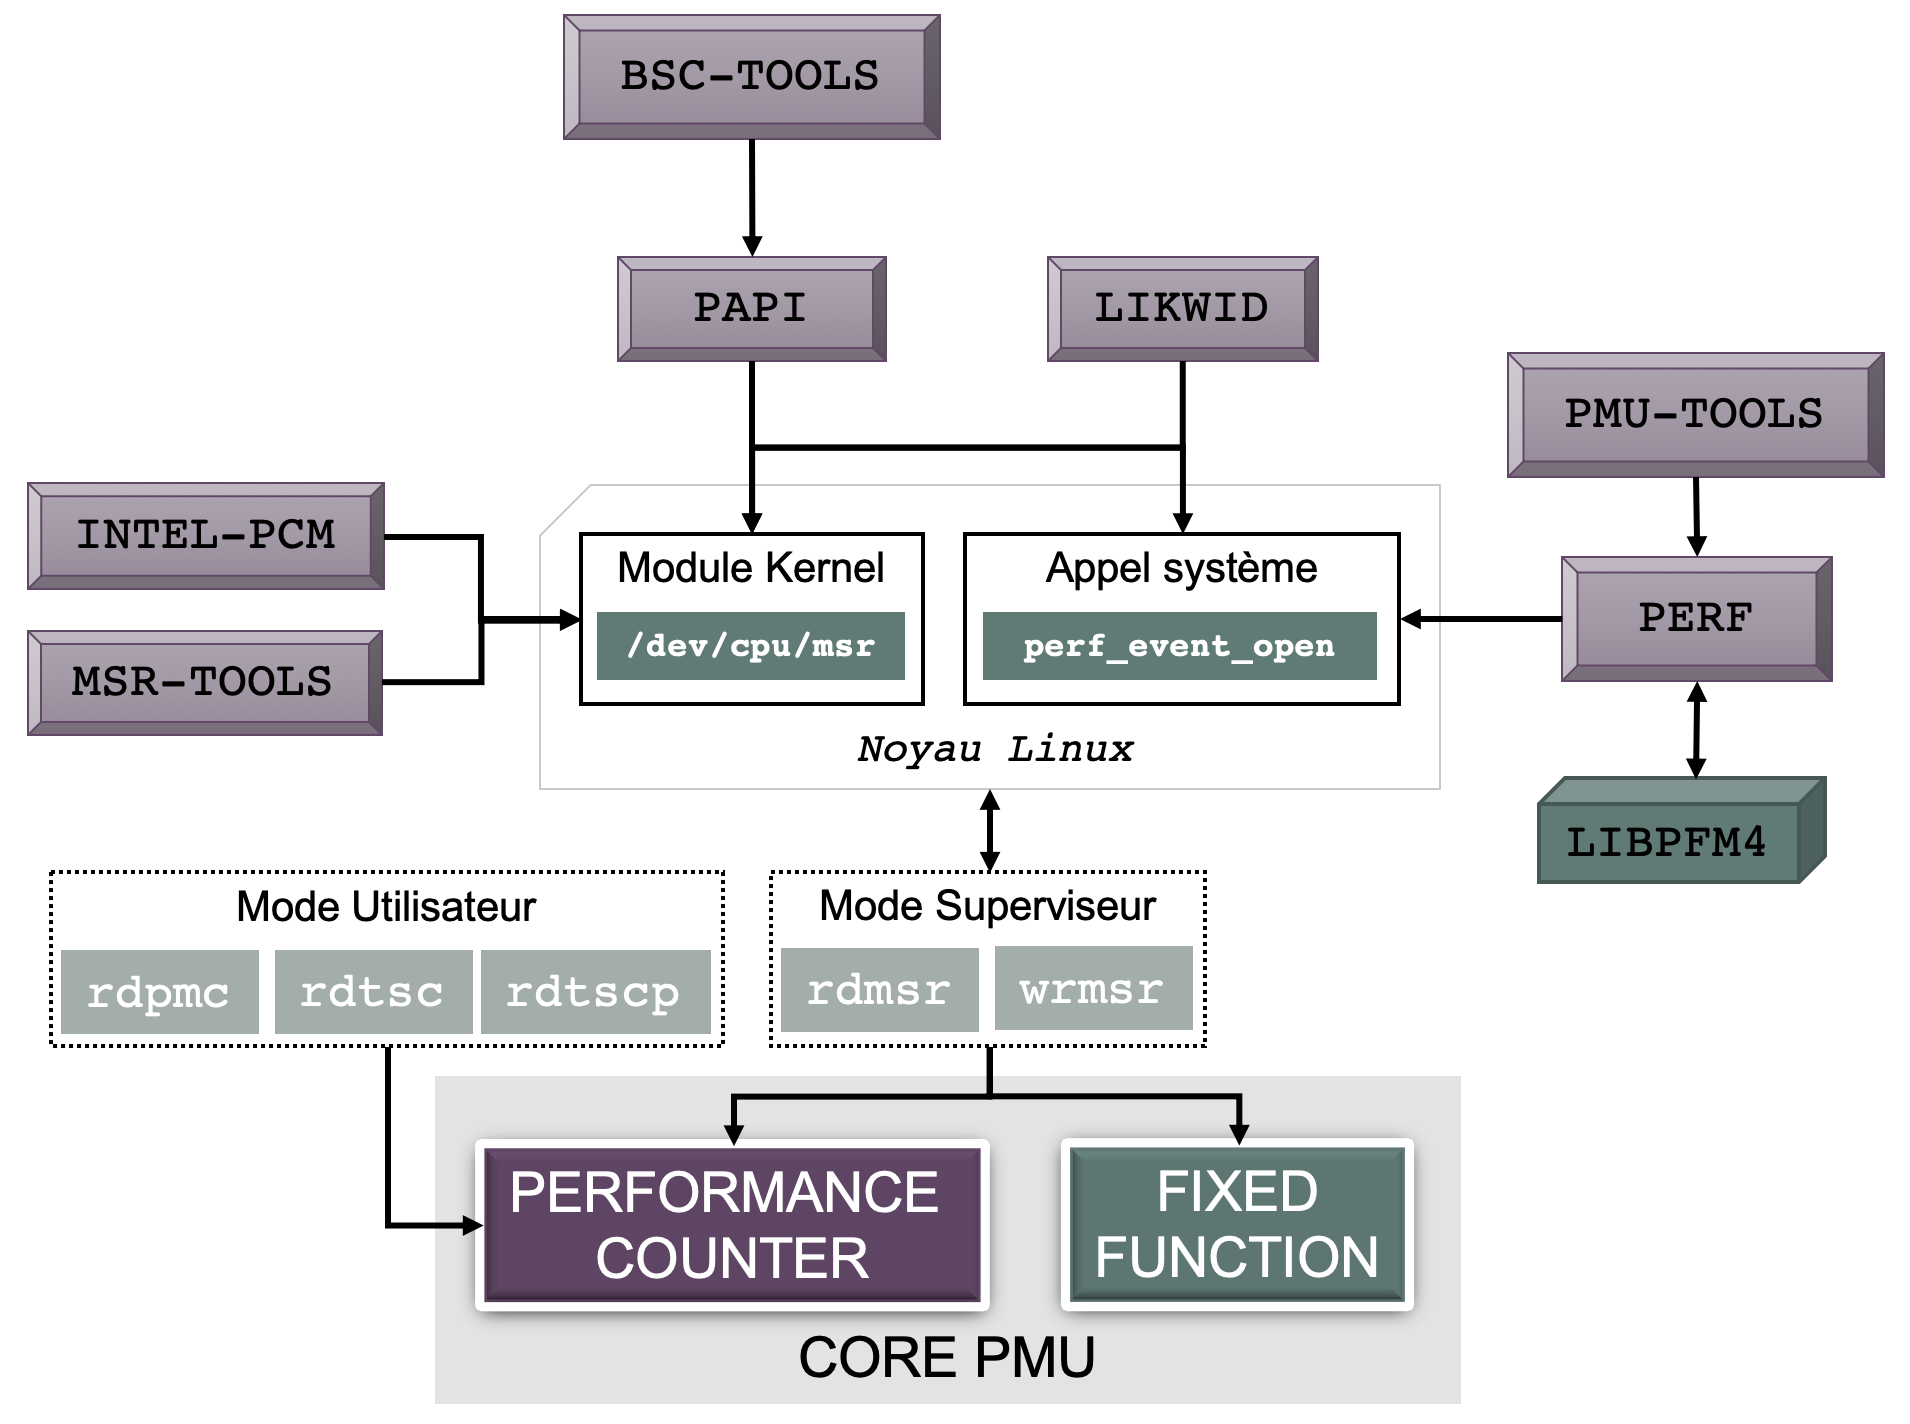
\includegraphics[width=14cm]{images/edl_perf_arbre.png}
            \caption{\label{fig:edl_perf_arbre} Différents moyens d'accéder aux compteurs localisés sur la PMU des coeurs. Linux propose deux interfaces permettant d'utiliser les deux instructions \textit{rdmsr} et \textit{wrmsr}: un module noyau et un appel système.}
            \end{figure}
 
 
        \subsubsection{Pseudo système de fichier /dev/cpu/CPUID/msr}
        %%%%%%%%%%%%%%%%%%%%%%%%%%%%%%%%%%        %%%%%%%%%%%%%%%%%%%%%%%%%%%%%%%%%%
            La première solution est implémentée par le noyau Linux et permet à l'utilisateur un accès bas niveau aux MSR sans avoir à utiliser de langages assembleurs. Ceci est réalisé à travers un pseudo système de fichier permettant d'interagir avec tous les coeurs (identifié par leur \verb|CPUID|) à travers le chemin \verb|/dev/cpu/#CPUID/msr|. Par défaut, seul l'utilisateur \textit{root} est autorisé à modifier ce fichier, mais ces droits peuvent être modifiés pour étendre l'accès aux autres utilisateurs. L'utilisation de cette interface est très pratique et peut être réalisée en accédant au fichier \textit{msr} grâce aux opérations \verb|pread()| et \verb|pwrite()|. Par exemple, pour lire le MSR dont l'adresse est \verb|0x38|, il suffit d'ouvrir le fichier \textit{msr} correspondant au coeur voulu, et réaliser une lecture avec un décalage de 38 octets.
            
            \begin{figure}[h!]
            \center
            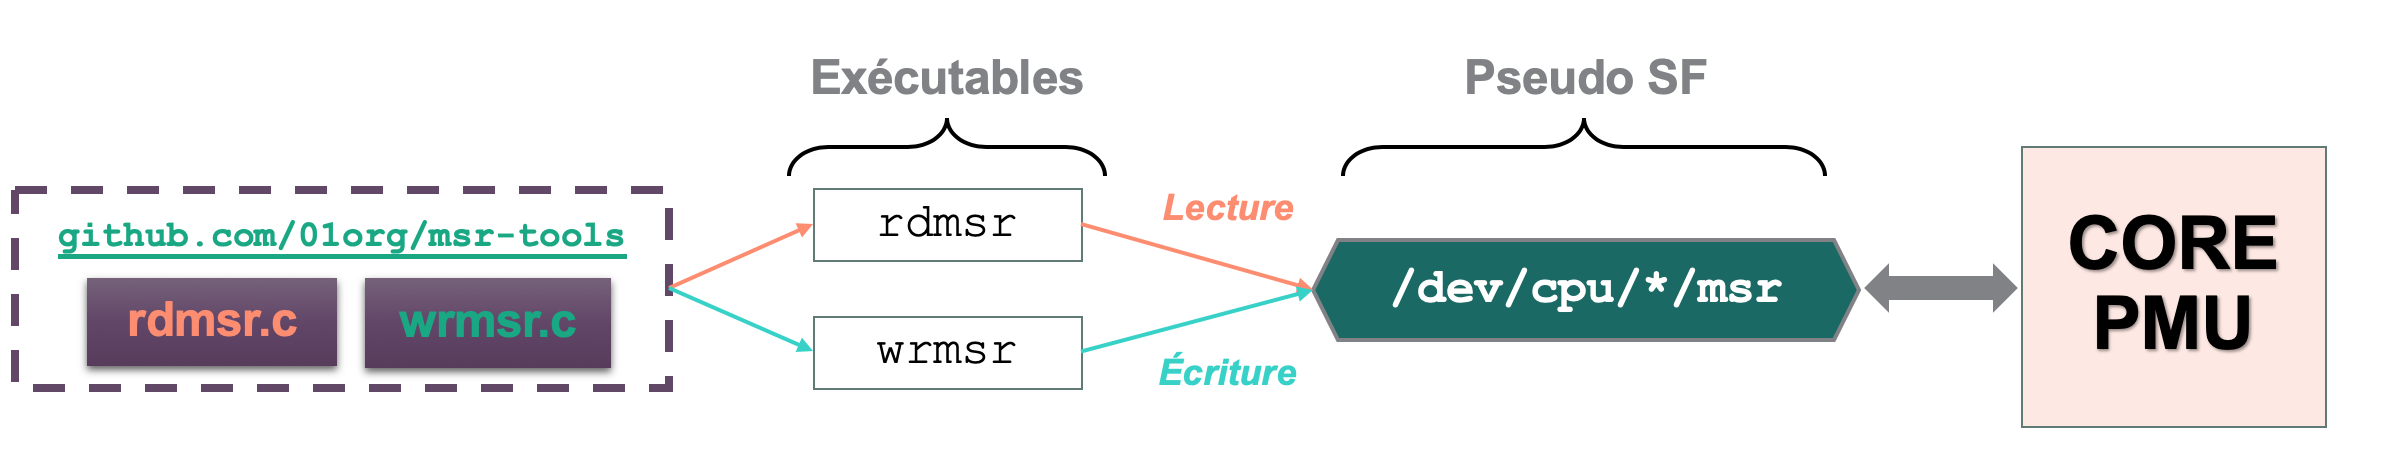
\includegraphics[width=14cm]{images/edl_perf_msrtools.png}
            \caption{\label{fig:edl_perf_msrtools} Intel propose deux exécutables permettant d'interagir plus facilement avec le pseudo système de fichier.}
            \end{figure}
        
            Pour faciliter l'usage de l'interface, Intel propose l'outil \textit{msr-tools} sur son GitHub\footnote{\url{https://github.com/intel/msr-tools}} (voir \autoref{fig:edl_perf_msrtools}).  La compilation produit deux exécutables \verb|rdmsr| et \verb|wrmsr| qui permettent de réaliser les lectures et écritures des registres MSR comme cela: \verb|./rdmsr -r 0x38D|. Nous proposons dans notre travail trois scripts permettant d'initialiser et configurer les compteurs grâce à ces deux programmes\footnote{\url{https://github.com/PourroyJean/performance_modelisation/tree/master/src/tool_PMU}}. 
    
    
        \subsubsection{Perfmon2}
        %%%%%%%%%%%%%%%%%%%%%%%%%%%%%%%%%%        %%%%%%%%%%%%%%%%%%%%%%%%%%%%%%%%%%
            Le projet perfmon2 était le principal candidat à l'inclusion dans le noyau Linux avant l'émergence surprise de \textit{Perf Events}. L'objectif du projet perfmon2 est de concevoir une interface générique de suivi des performances de bas niveau pour accéder à toutes les implémentations d'unités de surveillance des performances matérielles (PMU).
            
            L'interface utilise l'appel système \textit{perfmonctl}. Un appel système a été préféré à un driver de périphérique, car il offre une plus grande flexibilité et facilite la prise en charge par les implémentations d'un mode de surveillance par thread qui nécessite d'enregistrer et de restaurer l'état PMU du thread. L'interface exporte tous les registres PMU comme des registres 64 bits, même si de nombreuses implémentations PMU Interfaces en ont moins. L'interface ne sait pas ce que fait chaque registre, leur nombre, ni comment ils sont associés les uns aux autres. L'implémentation pour chaque plate-forme met en correspondance les PMC et PMD logiques sur les registres PMU réels. Toutes les informations spécifiques à un événement sont reléguées au niveau de l'utilisateur où elles peuvent être facilement encapsulées dans une bibliothèque.
        
            Le code de perfmon2 n'a jamais réussi à être inclus dans le projet Linux et son développement a été arrêté suite à la présentation du projet concurrent \textit{Perf Events}.
    
    
    
        \subsubsection{Perf Events}\label{sec:edl_profiling_perf}
        %%%%%%%%%%%%%%%%%%%%%%%%%%%%%%%%%%        %%%%%%%%%%%%%%%%%%%%%%%%%%%%%%%%%%
        
            Le projet de Compteur de Performance pour Linux (PCL) a été présenté en décembre 2008 et introduit dans Linux 2.6.31. Cet outil, rebaptisé ensuite \textit{Perf Events}, est une réponse au projet principal de standardisation des compteurs pour Linux de l'époque: perfmon2. Alors que ce dernier présentait beaucoup de fonctionnalités intéressantes, il n'a jamais réussi à être inclus dans le projet Linux. Lorsque \textit{Perf Events} fût ajouté au noyau Linux, de nombreuses fonctionnalités manquaient, mais sont apparues depuis. Pour fonctionner, \textit{Perf Events} utilise son interface \textit{perf\_event} développée directement dans le code du noyau Linux. Son adoption dans le noyau a mis un frein aux développements d'autres interfaces telles que \textit{perfmon2} ou \textit{perfctr} qui nécessitait de patcher le noyau pour être utilisée.  Du projet \textit{perfmon2}, seul la librairie \textit{libpfm4} est encore active. Il s'agit d'une librairie qui permet de convertir les noms symboliques d'évènements PMU en leur encodage pour \textit{Perf Events} ou d'autre interface noyau (exemple de la \autoref{fig:edl_perf_libpfm4}). La librairie en elle-même ne mesure aucun évènement. Elle fournit aux développeurs une interface pour lister, encoder les évènements pour beaucoup de PMU (core et uncore).
            
            \begin{figure}[h!]
            \center
            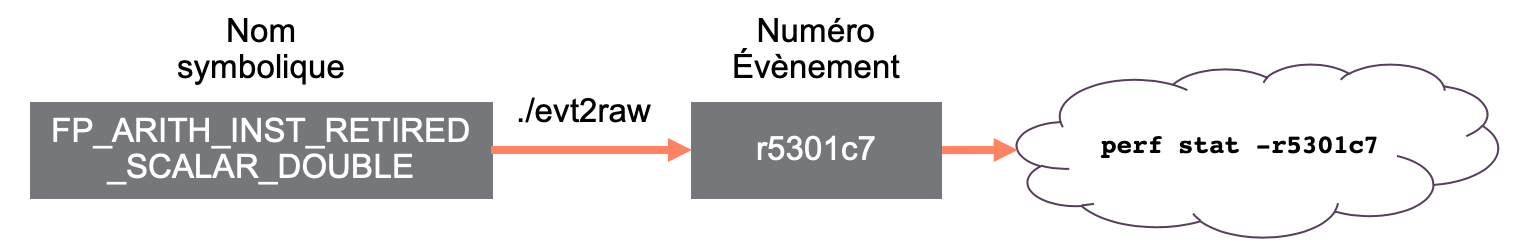
\includegraphics[width=12cm]{images/edl_perf_libpfm4.png}
            \caption{\label{fig:edl_perf_libpfm4} \textit{Libpfm4} permet de convertir les noms symboliques des évènements en leur encodage correspondant pouvant être utilisé avec des outils tels que \textit{perf}.}
            \end{figure}
            
            
            Un point de désaccord persistant entre \textit{Perf Events} et d'autres approches (tel que \textit{perfmon2}) est qu'il incorpore toutes les informations sur les compteurs et les événements dans le code du noyau lui-même, ajoutant ainsi une quantité significative de code descriptif au noyau. L'intégration de telles données dans le noyau peut causer des difficultés aux outils utilisateur pour prendre des décisions sur les événements qui peuvent être comptés simultanément et aux fournisseurs pour fournir des mises à jour sans avoir à patcher le noyau ou attendre de nouvelles versions du noyau. L'interface introduit un seul appel système comme point d'entrée (\textit{sys\_perf\_open}) qui renvoie un descripteur de fichier qui donne accès aux événements matériels. 
            
        
            \paragraph{perf.} 
            En plus de l'appel système, \textit{Perf Events} fournit un outil accessible depuis l'espace utilisateurs lui permettant de contrôler le profilage. Nommé \textit{perf}, ce programme utilise l'interface noyau pour réaliser des mesures soit en échantillonnage soit en comptage. Différentes commandes sont disponibles pour compter les évènements (\textit{stat}, \textit{record}, \textit{top}, \textit{bench}) et afficher les résultats (\textit{report}, \textit{annotate}). Grâce à la commande \textit{perf}, il est possible de compter les évènements en utilisant directement leur nom. La commande suivante peut être utilisée pour mesurer le nombre de transactions en lecture réalisées par un contrôleur mémoire. Il faut pour cela, vérifié que le noyau utilisé est capable d'accéder aux PMU uncore (première commande ci-dessous). Ensuite, il faut vérifier que le noyau supporte l'utilisation des noms d'évènements symbolique (deuxième commande ou \verb|perf list|). Enfin, la troisième commande permet de compter le nombre d'évènements.
            
    \begin{verbatim}
    #ls /sys/bus/event_source/devices/* | grep uncore_imc
    uncore_imc_0 uncore_imc_1 uncore_imc_3 uncore_imc_4 uncore_imc_5
    
    #ls /sys/bus/event_source/devices/uncore_imc_1/events/
    cas_count_read  cas_count_read.scale  cas_count_read.unit clockticks ...         
    
    #perf stat –a -e uncore_imc_0/cas_count_read/
    \end{verbatim}
            
            Malheureusement, lorsque les évènements voulus ne sont pas supportés par le noyau, il est nécessaire de se reporter à la documentation de l'architecture. Perf (comme PAPI) est capable de configurer les compteurs grâce à leur encodage (numéro de l'évènement, masque de configuration). Dans notre exemple, l'évènement est le numéro $0x04$ associé au masque $0x03$. Lorsque l'évènement est supporté par le noyau, c'est cette valeur qui est stockée dans les fichiers listés ci-dessus (première commande). Pour réaliser le même comptage que précédemment, la deuxième commande ci dessous peut être utilisée:

\begin{verbatim}
# cat /sys/bus/event_source/devices/uncore_imc_1/events/cas_count_read
event=0x04,umask=0x03

#perf stat -a -e "uncore_imc_0/event=0x04,umask=0x03/"
Performance counter stats for 'system wide':
4.94 MiB  uncore_imc_0/cas_count_read/
\end{verbatim}

    
           Le travail de Andy Kleen (\textit{pmu-tools}\footnote{pmu-tools: \url{https://github.com/andikleen/pmu-tools}}) peut aussi être utilisé pour faciliter l'utilisation de \verb=perf= lorsque les noms symboliques des évènements ne sont pas supportés. \verb=Ocperf= est un \textit{wrapper} de la commande \verb=perf= qui traduit les événements de la liste complète des événements Intel au format \textit{perf} lorsque ceux-ci ne sont pas supportés (première commande):

\begin{verbatim}
#perf  stat -e FP_ARITH_INST_RETIRED.128B_PACKED_DOUBLE sleep 1
invalid or unsupported event

#./ocperf.py  stat -e FP_ARITH_INST_RETIRED.128B_PACKED_DOUBLE sleep 1
perf stat –e cpu/event=0xc7,umask=0x4,name=fp_arith_inst_retired_128b_packed_double/ sleep 1
... correct ...
\end{verbatim}
                
    
            \paragraph{Avantages.} Bien qu'il s'agisse avant tout d'un outil d'espace utilisateur, la commande perf fait partie du noyau Linux du point de vue du développement. Faire partie de Linux assure une haute exigence du développement du code ainsi qu'un support au fil des versions du noyau. Lorsque le noyau supporte le nom symbolique des évènements, \textit{perf} est très simple à utiliser. Dans le cas contraire, \textit{Perf Events} offre la possibilité aux utilisateurs expérimentés d'encoder leurs propres évènements.
            
    
            \paragraph{Inconvénients.} L'inclusion de \textit{Perf Events} au projet Linux peut aussi être un inconvénient en rendant l'outil intrinsèquement lié à la version du noyau Linux. Ceci implique que pour utiliser les nouvelles fonctionnalités de perf il faut généralement installer la version du noyau correspondante. La deuxième difficulté vient de l'appel système \textit{perf\_event\_open}. S'il permet d'éviter à l'utilisateur d'écrire manuellement les différents bits de configuration des MSR, beaucoup de travail reste à faire pour le développeur désireux de profiler ses applications. Parce que Linux supporte de nombreux processeurs différents possédant différentes versions de PMU, les développeurs de noyau ont dû laisser la charge de beaucoup de détails de microarchitecture de bas niveau dépendant du code utilisateur. En conséquence, cet appel système est très complexe à utiliser et ne peut pas être utilisé de manière portable. Les principales difficultés consistent à trouver les événements à compter ou à échantillonner, à configurer tous les paramètres à transmettre à l'appel système et à effectuer plusieurs appels système en fonction du nombre de \textit{threads} de l'application profilée et du nombre de coeurs utilisés. Ces différentes difficultés (programmation, portabilité) ont été les principales motivations du développement d'autres outils tels que PAPI, Intel Performance Counter Monitor (PCM) ou NUMAP\cite{Selva2017}.


        \subsubsection{Oprofile.} 
        %%%%%%%%%%%%%%%%%%%%%%%%%%%%%%%%%%        %%%%%%%%%%%%%%%%%%%%%%%%%%%%%%%%%%
            Oprofile \cite{Levon2004} est un outil de suivi de performance développé par John Levon en 2001 dans le cadre de son projet de master et fut le principal outil de suivi de performance de Linux pendant plusieurs années\footnote{source: \url{https://www.ibm.com/developerworks/linux/library/l-evaluatelinuxonpower/}}. 
            Oprofile est capable d'utiliser des compteurs de performances matérielles pour suivre la performance des processus, des bibliothèques partagées et du noyau. Pour suivre ces performances, Oprofile utilise un démon permettant à l'utilisateur de spécifier un événement matériel à surveiller et un seuil d'événement pour déclencher l'interruption (échantillonnage). En utilisant les tables de symboles de débogage, il peut faire le lien entre les adresses des instructions et les lignes du code source associées. Oprofile est un outil mature possédant une multitude d'option telle que la génération de graphiques d'appel (\textit{call graph}). Plusieurs utilitaires sont fournis à l'utilisateur pour contrôler le suivi de performance (\textit{opcontrol}, \textit{opreport} ...).
            A l'origine, Oprofile utilisait un module noyau nécessaire pour accéder aux PMU. Quand \textit{Perf Events} fut introduit avec son interface noyau, Oprofile a alors été adapté pour l'utiliser lui aussi. La communauté autour de la commande \verb|perf| est sans doute plus active et dynamique, et de nombreuses nouvelles fonctionnalités sont ajoutées à \textit{perf} sans analogies dans \textit{OProfile}.
    
        \subsubsection{PAPI}
        %%%%%%%%%%%%%%%%%%%%%%%%%%%%%%%%%%        %%%%%%%%%%%%%%%%%%%%%%%%%%%%%%%%%%
            L'interface Performance Application Programming Interface (PAPI), a pour objectif de simplifier l'utilisation des PMUs de différentes architectures. Pour cela, PAPI offre une abstraction pour un grand nombre de compteurs d'évènements pour le développement d'outils de suivi de performance. Pour accéder aux MSR, PAPI utilisait l'interface \textit{perfctr} avant de basculer sur l'interface offerte par \textit{Perf Events} avec la version 2.6.32 du noyau Linux. PAPI supporte le comptage, l'échantillonnage ainsi que le multiplexage. Utiliser la totalité des fonctionnalités de PAPI nécessite une certaine expérience. Cependant pour un usage basique, son utilisation est très simple comme le montre l'exemple de l'\autoref{lst:edl_perf_pai}.

\begin{lstlisting}[
label=lst:edl_perf_pai,
basicstyle={\scriptsize\ttfamily},
identifierstyle={\color{black}},
language={c},
tabsize=2,
numbersep=8pt,
frame=tlbr,framesep=2pt,framerule=0pt,
morekeywords ={class,run},
caption=Utilisation simple de l'API PAPI pour mesurer deux évènements dans un programme C.
]
#define NUM_EVENTS 2  
long_long values[NUM_EVENTS];
unsigned int Events[NUM_EVENTS]={PAPI_TOT_INS,PAPI_TOT_CYC};
PAPI_start_counters((int*)Events,NUM_EVENTS); /* Start the counters */
do_work();
PAPI_stop_counters(values,NUM_EVENTS); /* Stop counters and store results*/
\end{lstlisting}

        
            PAPI est composé de deux parties permettant de compter des évènements dits \textit{natifs} ou \textit{prédéfinis}. 
            
            \paragraph{Les événements \textbf{natifs}} comprennent l'ensemble des événements qui peuvent être comptés par le CPU. Dans de nombreux cas, ces événements seront disponibles par le biais d'un événement PAPI prédéfini correspondant. Il y a généralement beaucoup plus d'événements natifs disponibles qu'il n'est possible d'en mapper sur des événements prédéfinis du PAPI. Même si aucun événement prédéfini n'est disponible, les événements natifs sont toujours accessibles directement. L'utilisation de ces évènements nécessite d'avoir une bonne connaissance de l'architecture utilisée. Chaque évènement peut être configuré grâce à un \textit{masque} pour désigner précisément l'évènement à compter de la même façon que lors de la programmation des MSR grâces aux commandes \textit{rdmsr} et \textit{wrmsr} présentées dans la \autoref{sec:perf_asm_msr}. 
            
            \paragraph{Les événements \textbf{prédéfinis}} sont un ensemble commun d'événements jugés pertinents et utiles pour le réglage des performances des applications. Ces événements se trouvent généralement dans de nombreux CPU qui fournissent des compteurs de performance et donnent accès à la hiérarchie de la mémoire, aux événements du protocole de cohérence du cache, au nombre de cycles et d'instructions, à l'unité fonctionnelle et au statut du pipeline. En outre, les événements prédéfinis sont des mappages de noms symboliques (nom prédéfini du PAPI) à des définitions spécifiques à la machine (événements natifs). Par exemple, le nombre total de cycles passés en mode utilisateur est PAPI\_TOT\_CYC\footnote{source:\url{https://icl.cs.utk.edu/projects/papi/wiki/Events}}. Un évènement prédéfini peut utiliser une combinaison d'un ou plusieurs évènements natifs permettant de compter un évènement prédéfini. Par exemple, l'évènement pour compter le nombre de calculs flottants simple précision exécuté peut être mesuré avec l'événement prédéfini \textit{PAPI\_SP\_OPS}. Cet évènement utilise en réalité quatre évènements natifs pour compter les instructions vectorielles de différentes tailles pour ensuite calculer le résultat \textit{Number of FLOPS}.

\begin{verbatim}
#papi_avail -e PAPI_SP_OPS
    Number of Native Events:      4
    Long Description:            |Single prec. op; vector|
    Postfix Processing String:   |N0|N1|4|*|+|N2|8|*|+|N3|16|*|+||
    Number of FLOPS= N0 + N1 * 4 + N2 * 8 + N3 * 16
\end{verbatim}

            Il y existe une centaine d'évènements prédéfinis par PAPI. La disponibilité de ces derniers peut être vérifié grâce à la commande \verb|papi_avail|. Il est possible de créer ses propres jeux d'évènements prédéfinis. En raison des différences d'implémentation matérielle, il n'est pas toujours possible de comparer directement les comptes d'un événement prédéfini par PAPI obtenu sur différentes plates-formes matérielles.

    
        %%%%%%%%%%%%%%%%%%%%%%%
        \subsubsection{Likwid}
        
            LIKWID est un ensemble d'outils utilisable en ligne de commande pour aider les développeurs dans leur travail de caractérisation de plateformes et d'analyse de performances. Les outils fonctionnent sur la majorité des distributions Linux grâce à sa faible dépendance de libraires externes: il ne nécessite que le compilateur \textit{GNU compiler}. L'outil possède 11 outils pouvant être groupés en trois catégories: analyse de performance, caractérisation de plateforme et contrôle de l'exécution. Les outils de caractérisation sont présentés dans la \autoref{sec:likwid_bench}. Deux outils sont importants pour analyser les performances d'une application: \textit{likwid-perfctr} et \textit{likwid-perfscope}.
        
            Le premier permet d'accéder aux compteurs de performances à travers les interfaces principale telles que \textit{Perf Events} ou \textit{perf\_ctr}. Les principaux évènements sont accessibles (\textit{core} et \textit{uncore}) et la majorité des processeurs x86 sont supportés grâce au sous-système \textit{perf\_event\_open()} (Intel Xeon, Intel Xeon Phi, et AMD Zen). L'avantage de cet outil est de pouvoir utiliser des groupes d'évènements déjà existants tels que.:
\begin{lstlisting}
FLOPS_SP   Operation flottante simple precision MFlops/s
L3         Bande passante du cache L3 en MBytes/s
MEM        Bande passante mémoire en MBytes/s
\end{lstlisting}
            L'outil peut être utilisé pour mesurer la performance d'un système ou d'une application particulière utilisant la programmation multi-coeur. 
        Likwid propose une API permettant d'annoter le code pour ne mesurer la performance que de certaines régions de l'application:
\begin{lstlisting}
LIKWID_MARKER_START(Compute);
<code>
LIKWID_MARKER_STOP(Compute);
\end{lstlisting}
            Pour pouvoir fonctionner, l'application doit être compilée avec le drapeau de compilation \verb|-DLIKWID_PERFMON|. L'avantage est de pouvoir facilement désactiver la mesure de performance et n'ajouter aucun coût supplémentaire à l'application lors d'une utilisation en production.
        
        
            Le deuxième outil, \textit{likwid-perfscope}, est un outil de visualisation des données mesurées par le premier. Il permet par exemple d'afficher l'évolution du trafic mémoire lors de l'exécution de l'application ou de la consommation énergétique. Malheureusement, cet outil n'est pas supporté pour les processeurs Skylake. Après avoir discuté avec le développeur de cette application, il semble que cet outil soit un "\textit{jouet}" et que le développeur originel ne fasse plus partie du projet.  
            
        \subsubsection{BSC Performance Tools}
        Le centre de recherche du Barcelona Supercomputing Center développe depuis 1991 une suite d'outil permettant la caractérisation des applications. 
        
        Cette suite d'outils est principalement composée de trois outils: \textit{Extrae} \cite{Rodriguez}, \textit{Paraver} \cite{Pillet1995} et \textit{Dymemas} \cite{Labarta1997}. La philosophie d'utilisation de ces outils est d'aider l'utilisateur à trouver le goulot d'étranglement des performances de son application qui peut être dû à plusieurs facteurs. Les outils ne sont pas une boîte noire répondant à toutes les questions automatiquement. La méthodologie d'analyse, comprenant l'utilisation de \textit{Paraver} et \textit{Dimemas}, est basée sur l'examen de la distribution temporelle et spatiale des données de performance pour comprendre le comportement de l'application, détecter ses différentes phases et identifier la structure comportementale (qui peut être différente de la structure procédurale). Cette analyse détaillée permet d'extraire beaucoup d'informations des données de performance recueillies au cours de l'exécution. L'utilisateur doit être un programmeur confirmé dans l'analyse de performance et utiliser les outils pour l'aider dans son analyse de performance. Les outils permettent de facilement comparer plusieurs traces correspondant à différentes exécutions de l'application (paramètres ou architectures différents). 
        
        L'outil \textit{Extrae} signifie \textit{extraire}. Il permet notamment d'instrumenter dynamiquement un code pour en extraire des traces qui pourront être visualisées avec l'outil \textit{Paraver} (\textit{pour voir}). L'outil injecte une librairie (\verb=LD_PRELOAD=) pour annoter les différents symboles de l'application. La librairie \textit{Dyninst} est utilisée pour réaliser l'instrumentation au niveau du code source ou directement dans le binaire. L'ensemble des outils est compatible avec \textit{OpenMP} et \textit{MPI} pour permettre d'obtenir des profils d'exécution parallèle. La \autoref{fig:edl_perf_paraver} montre un exemple de deux traces dont les graphiques sont alignés pour faciliter l'extraction de résultats. La première fenêtre montre en rouge les appels à des fonctions de communication de la librairie \textit{MPI}. Les parties en noire représentent le code de l'application propre à chaque coeur. La deuxième fenêtre montre à l'aide d'un dégradé de couleur le nombre d'instructions utiles par cycle. Les couleurs claires représentent un \textit{IPC} plus faible. On remarque ainsi que les communications ne sont pas parfaitement synchrones et que des coeurs perdent un certain temps à attendre que les autres coeurs aient fini leur partie du travail. L'outil \textit{Paraver} possède une visualisation sous forme de tableur permettant de quantifier le temps perdu à cause de ces désynchronisations et d'identifier le nom des fonctions responsables.  
        
        \begin{figure}
        \center
        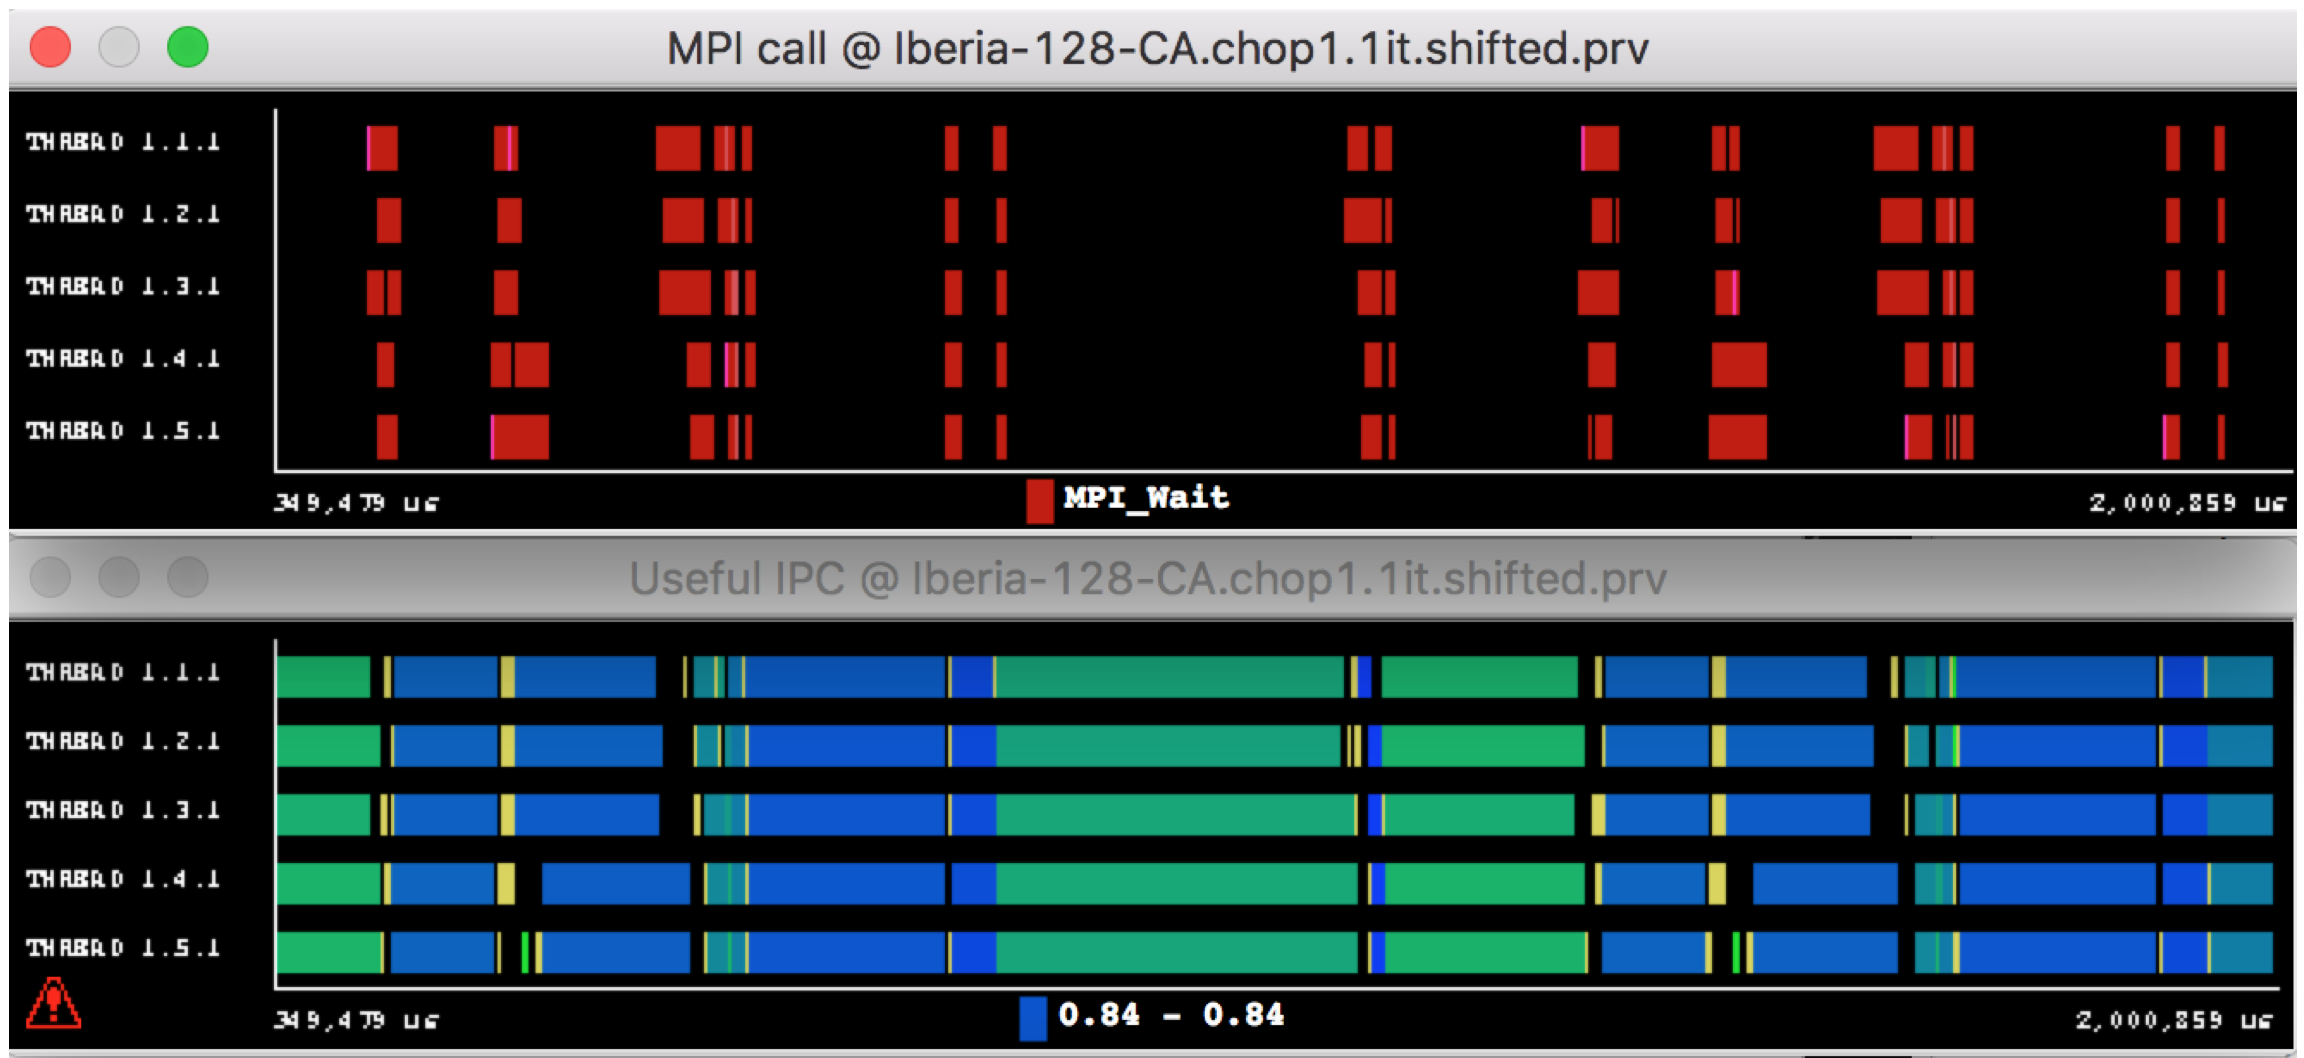
\includegraphics[width=12cm]{images/edl_perf_paraver.png}
        \caption{\label{fig:edl_perf_paraver} L'outil \textit{Paraver} permet d'afficher le graphique des traces obtenues grâce à l'outil \textit{Extrae}.}
        \end{figure}
        
        Le troisième outil, \textit{Dimemas}, permet à l'utilisateur de développer et optimiser des applications parallèles sur son poste de travail, tout en fournissant une prédiction précise de leurs performances sur une architecture parallèle. Le simulateur Dimemas reconstruit le comportement temporel d'une application parallèle sur une machine modélisée par un ensemble de paramètres de performance. Ainsi, les expériences de performance peuvent être faites facilement. L'absence de latence du réseau (virtuel) permet d'estimer les performances de son application si elle utilisait un supercalculateur avec un réseau parfait. L'utilisateur peut ensuite estimer l'impact apporté par le portage sur MPI et OpenMp. Les traces générées par \textit{Dimemas} peuvent ensuite être analysées avec l'outil \textit{Paraver}.



\subsection{Conclusion}\label{sec:edl_hc_conclusion}
%%%%%%%%%%%%%%%%%%%%%%%%%%%%%%%%%%
    
    \subsubsection{Discussion}
    
        %%%%%%%%%%%%%%%%%
        \paragraph{Documentation.}
            La principale difficulté pour l'utilisation des compteurs matériels est le manque de connaissance des utilisateurs et leur faible documentation. La documentation des évènements est critique, car l'utilisateur doit être assuré qu'il mesure bien la valeur souhaitée et nous pouvons regretter la mauvaise documentation des compteurs qui est souvent vague pour que l'utilisateur n'ait pas d'attente erronée de ce qu'il peut mesurer. Ce manque de documentation à un grand impact sur la quantité et la qualité des outils disponibles. Nous pouvons aussi regretter que ce manque oblige de nombreux programmeurs à pratiquer de la rétro-ingénierie pour comprendre certains comportements de la microarchitecture ou de l'utilisation des compteurs.

            Utiliser directement les compteurs est en effet difficile. Il est nécessaire de connaître l'adresse des compteurs, de savoir comment les configurer (numéro de l'évènement, masque) et enfin d'interpréter les résultats. Ce travail est conséquent, car ces informations se trouvent dans de longues documentations (celle d'Intel fait plusieurs milliers de pages). Aussi, les descriptions de ces événements ne sont pas tout le temps clair, et trouver le bon évènement est complexe. Dans la même documentation, le même compteur peut être référencé avec le préfixe \verb=IA32_= ou \verb=MSR_= et certains registres MSR peuvent changer de nom d'une architecture à l'autre, rendant la recherche d'autant plus difficile. Certains détails des PMU Skylake (version 3) sont à aller chercher dans la version 1 plusieurs dizaines de pages avant, pour ensuite comprendre qu'elles ont été modifiées dans la version 2. De plus la documentation est incomplète, certains compteurs n'y apparaissent pas. Par exemple les compteurs \textit{uncore} utilisés pour mesurer la bande passante mémoire ont été rendus publics plusieurs mois après dans une documentation séparée.
      
            Face à ce manque de documentation il est légitime de se demander pourquoi celle-ci n'est pas réalisée avec plus de consistances. Un premier argument  peut être de protéger la confidentialité de certaines implémentations du processeur. Une autre explication peut aussi venir de la vente de licences des outils propriétaire des constructeurs qui s'assurent une faible concurrence. Cependant, après de nombreux échanges avec les architectes de processeurs Intel, il semble que la principale raison soit technologique. Ajouter des compteurs implique l'utilisation de transistors supplémentaires (et donc d'énergie) pour une utilisation autre que l'amélioration de la performance du processeur. A l'inverse, l'ajout de compteurs aura un impact sur la performance des applications, notamment aux endroits sensible tels que les caches. Les constructeurs semblent réticent à l'idée de substituer ces transistors qui peuvent être utilisés pour le développement d'autres matériels du processeur. Il est important de rappeler que ces compteurs ne sont à l'origine crées que pour des usage de deboguage. Les constructeurs construisent alors le sous-ensemble minimum de compteurs leur permettant de vérifier le bon fonctionnement de la microarchitecture.
            


            
            
        %%%%%%%%%%%%%%%%%
        \paragraph{Droits}
            L'accès aux compteurs n'est possible qu'en utilisant les instructions \verb=rdmsr= et \verb=wrmsr=. Pour des raisons de sécurité, il semble évident que de laisser l'accès à ces informations aux utilisateurs est dangereux notamment lorsque les processeurs sont partagés entre plusieurs utilisateurs. L'obligation d'avoir des droits privilégiés pour utiliser les compteurs est un frein au développement d'outils, mais aussi à l'utilisation de ces compteurs. En effet, dans des environnements tels que les centres de calculs, il est rare que les utilisateurs possèdent ce niveau de droits. Bien que ce soit rare dans le domaine du HPC, les centres de données ont de plus en plus recours à la virtualisation ou à la dockerisation. L'ajout de cette couche rend d'autant plus complexes l'accès et la valorisation de ces compteurs. 
            Heureusement, des interfaces ont été développées pour donner l'accès aux compteurs aux utilisateurs standard. Les versions récentes du noyau Linux offre une abstraction à travers le pseudo système de fichier \verb=/dev/cpu/CPUID/msr= qui permet d'écrire et lire les compteurs. 
     
     
        %%%%%%%%%%%%%%%%%
        \paragraph{Évolution du matériel.}
            Au vu de la forte demande et attente des utilisateurs des compteurs matériels, nous remarquons que dans les dernières années les capacités des PMUs ont faiblement évolué \cite{Intel2017}. Un exemple marquant du manque d'implication des constructeurs fut la disparition d'un compteur majeur permettant de mesurer le nombre d'opérations flottantes exécutées sur l'architecture Haswell.

            Face au faible développement matériel, la partie logiciel a dû évoluer pour proposer de nouvelles fonctionnalités. Par exemple, le multiplexage des évènements aurait pu être directement réalisé par la PMU. Aussi, nous constatons une explosion des outils existants qui redouble d'inventivité pour aller chercher des informations toujours plus pointues (Likwid \cite{Treibig2011}, TAU \cite{Shende2006}, Perf \cite{Weaver2013}, Extrae \cite{Markomanolis2014} … ). 

            Certaines études \cite{Moseley2011} proposent même d'abandonner les compteurs matériels au profit d'outils seulement logiciel comme Pin tool d'Intel \cite{RobertD.2011} ou Dyninst \cite{RobertD.2011, Laurenzano2012}. Le challenge n'est plus alors de récupérer les donner qui peuvent être fait à faible impact (moins de 1\% grâce à des techniques de \textit{shadow profiling} ou \textit{brusty tracing} \cite{Moseley2011}) mais plutôt dans l'analyse de ces traces. L'utilisation de techniques d'apprentissages peut alors être une bonne piste pour valoriser ces données. \cite{Moseley2011} explore des pistes où ces collections et analyses de traces seraient la clef. Les traces collectées par les clients seraient alors envoyées au constructeur pour les analyser et simuler de potentielles performances sur des architectures qui n'existent pas encore. Cela simplifierait les échanges avec les clients qui sont souvent réticents à sortir les jeux de données de leur centre.

        %%%%%%%%%%%%%%%%%
        \paragraph{Impacte sur la performance}
        
            L'incrémentation des compteurs de performance n'affecte pas (ou peu \cite{Rohl2015}) la performance de l'application étudiée. L'impact sur la performance vient de l'extraction de ces valeurs pour pouvoir être traité. Comme dans tout système physique, l'acte de mesurer perturbe le phénomène mesuré. Les accès aux compteurs à travers des interfaces introduisent nécessairement des coûts sous la forme d'instructions supplémentaires (y compris les appels système), et les interfaces provoquent une pollution du cache qui peut modifier le comportement du cache et de la mémoire de l'application surveillée \cite{Weaver2015}. Les bibliothèques telles que PAPI ajoutent aussi des instructions à exécuter chaque fois qu'une routine est appelée, ce qui peut apparaître dans les résultats du compteur. 
            
            Certains travaux ont été menés pour mesurer le coût de l'utilisation des compteurs matériel \cite{Bitzes2014}. Les résultats montrent que le coût varie fortement en fonction des événements étudiés, de la fréquence d'accès aux compteurs, du nombre d'événements et surtout de l'utilisation du mode d'échantillonnage. L'impact principal sur la principale est mesuré lors de l'utilisation du multiplexage. Il est notamment souvent recommandé de ne pas utiliser plus d'événements qu'il n'y a de compteurs matériels disponibles, en particulier en mode échantillonnage. Sinon, le coût engendré peut atteindre jusqu'à 25\% d'augmentation du temps d'exécution de l'application. Ce résultat suggère qu'il y a encore de la place pour l'optimisation des interfaces d'accès aux compteurs. 
    
        %%%%%%%%%%%%%%%%%
        \paragraph{Validation des évènements}
        
            Pour pouvoir tirer des conclusions des résultats mesurés par les compteurs il est nécessaire de réaliser deux validations: la première est de s'assurer que l'évènement utilisé mesure bien le comportement souhaité, la deuxième est de valider le bon comportement du compteur.
        
            Les valeurs reportées par les compteurs peuvent fortement varier entre deux exécutions de la même application. Même si un programme est spécifiquement conçu pour être déterministe, d'autres facteurs peuvent causer différents comptages (espace d'adressage différent, autre application utilisant une ressource partagée comme le cache). Le biais est une grande difficulté à appréhender lorsque les mesures peuvent varier d'un facteur trois pour la même application.
                
            La vérification des évènements est quasi inexistante aujourd'hui. Ces efforts sont souvent réalisés en interne et la communauté \cite{Moseley2011} peut regretter l'inexistence de projet libre mettant en commun différents microbenchmarks permettant de valider précisément le bon fonctionnement des compteurs pour un ensemble d'évènements. \cite{Moseley2011} avance une idée pour les valider qui serait d'écrire un microbenchmark par évènement pour le stresser et avoir une fourchette des valeurs atteignables. Plusieurs travaux sont présentés dans leur papier pour valider les compteurs de miss du cache L1 en utilisant plusieurs compteurs censés les mesurer. Ils ne sont pas parvenus à atteindre les résultats attendus.
        
            
         %%%%%%%%%%%%%%%%%
        \paragraph{Interprétation des résultats}
            En admettant que l'on soit capable de récupérer les valeurs exactes associées aux compteurs, il reste encore des difficultés avant de comprendre le comportement de l'application. Les informations sous forme de ratio comme « nombre de miss par cycle » sont très dures à interpréter et nous pouvons nous demander à partir de quelle valeur elle peut être considérée comme bonne ou mauvaise. Une idée pourrait être de définir des compteurs et leur associer des bonnes ou mauvaises valeurs, mais \cite{Moseley2011} fait remarquer que c'est un challenge. Intel PMT \cite{RobertD.2011} utilise des techniques d'apprentissages pour corréler la valeur des compteurs avec les instructions exécutées.
            
             
                
    
    \subsubsection{Conclusion}
    %%%%%%%%%%%%%%%%%%%%%%%%%%%%%%%%%%

        Les compteurs matériels de performance sont un outil puissant qui permet d'avoir un aperçu du comportement des microarchitectures qui se sont grandement complexifiées ces dernières années. Ce travail de thèse s'intéresse aux compteurs matériels pour deux raisons principales: l'analyse des performances et l'optimisation des applications. L'objectif de cette section est de réaliser un état de l'art des outils existant pour notre démarche. L'utilisation des compteurs matériels a de nombreux avantages, mais aussi des limites qui empêchent l'automatisation de l'analyse de performance. 

        \paragraph{Avantages.} Le premier avantage des compteurs matériel est d'être implémentés directement par le processeur sans quoi il serait impossible de suivre précisément l'activité de la microarchitecture (\textit{miss} dans les caches, remplacement dans la TLB, nombre de cycles exécuté). Il faudrait pour cela utiliser des simulateurs dont les résultats sont souvent différents des performances réelles des processeurs réels. La seule tâche du programmeur est de configurer les compteurs et consulter leur valeur pour réaliser son étude.
        Nous avons montré que depuis l'apparition des compteurs matériels, une multitude d'interfaces et d'outils permettant d'y accéder ont été développés. L'utilisation d'outils tels que le \textit{PAPI} ou \textit{Perf Events} peut grandement améliorer la compréhension et permettre d'améliorer la performance de codes difficiles à comprendre. 
        À l'origine, les compteurs matériels n'étaient pas destinés aux utilisateurs de processeurs. Cependant, leur présence et les efforts réalisés par la communauté a permis d'en dériver de nombreuses utilisations: \cite{Moseley2011} optimisation guidé par profile\cite{Cavazos2006a}, optimisation dynamique\cite{Dai2005}, adaptation de la gestion de l'énergie \cite{Isci2005}, ordonnancement des \textit{threads} pour les ressources partagées\cite{Moseley2006} et autres \cite{Shye2005, Shye2008}.
        
        \paragraph{Inconvénients.} Si l'utilisation de compteurs matériels a de nombreux avantages, elle comporte aussi des inconvénients majeurs empêchant leur pleine utilisation. 
        La première difficulté rencontrée vient de la complexité de programmation des compteurs. Pour accéder à ces compteurs, il faut développer du code bas niveau, assembleur/c. Ce code varie d'un modèle de processeurs à l'autre rendant difficile sa portabilité. Le code bas niveau nécessaire pour leur programmation nécessite une lecture attentive de la documentation du constructeur qui fait plusieurs milliers de pages et qui n'est pas toujours complètes. Des architectures récentes comme les processeurs Intel Skylake possèdent des dizaines de compteurs permettant de suivre l'activité des contrôleurs mémoires. La sélection du compteur approprié pour résoudre un problème en particulier est loin d'être trivial, notamment dû au manque de documentation de ceux-ci.
        Aussi, la majorité des évènements des architectures Intel sont considérés comme non architecturaux. Intel ne garantit pas que ces compteurs soient maintenus dans les prochaines versions de processeur. Cette particularité est une raison majeure du renoncement des développeurs à écrire et/ou à maintenir des outils qui pourraient ne plus être utilisables sur l'architecture suivante.
        Pour notre travail, la deuxième difficulté est de trouver des outils portables sur des architectures différentes dont la communauté soit suffisamment active pour porter leur développement. Certains outils fonctionnels ont été développés il y a plusieurs années, mais l'effort de portage n'a jamais été réalisé. Ce critère est essentiel dans le choix des outils utilisés dans notre travail qui a pour ambition de pouvoir être appliqué sur des architectures de différents constructeurs.
        Un autre problème des compteurs matériels vient de leur manque de précision. À cause de la grande évolution de la complexité des architectures, l'attribution des évènements au code responsable est loin d'être évidente. Les processeurs utilisant des pipelines superscalaires et des tampons d'exécution dans le désordre rendent difficile la caractérisation fine du comportement d'un code. Ce frein implique d'utiliser des méthodes de validation des compteurs pour vérifier qu'il compte bien le nombre d'évènements attendus. Nous recommandons ainsi de toujours valider les compteurs avant de tirer une conclusion sur la performance d'un code. Des outils tels que \textit{X86-membench}\cite{Molka2017} ont été développés dans cet objectif pour les compteurs relatifs aux l’accès mémoire, mais doit être étendu à la totalité des évènements.
        La validation du comportement des compteurs est une première étape, mais il faut ensuite pouvoir en comprendre la signification. À partir de quel seuil le nombre d'évènements mesuré est-il problématique ? Par exemple, un grand nombre de \textit{miss} dans le premier niveau de cache, n'implique pas forcément que le code est de mauvaise qualité. Par exemple, un algorithme de \textit{streaming} doit avoir un grand nombre de miss, il faudrait par exemple corréler l'utilisation du bus entre le cache de niveau un et deux pour conclure à une mauvaise performance. En plus d'utiliser la valeur d'un compteur, il est intéressant d'utiliser des ratios d'évènement tel que le nombre de \textit{miss} par instructions exécutées ou du nombre d'instructions flottantes exécutées par cycle. La documentation manque aussi de préciser quelle valeur constitue le ratio d'une application ayant une bonne/mauvaise performance. Ce genre de raisonnement peut être appliqué à la majorité des évènements mesurables. 
        
        \paragraph{Choix d'un sous-ensemble d'évènements.} Les avantages et les inconvénients résumés ici étaient pour la majorité déjà actuels en 2002 \cite{sprunt2002basics}. Ce domaine ayant peu évolué depuis toutes ces années, nous devons nous satisfaire de l'état actuel de ces technologies sans espérer d'amélioration. Les outils développés dans le cadre de cette thèse ont pour objectif d'être utilisés sur des architectures très différentes. Pour cette raison, nous avons décidé de restreindre le nombre d'évènements nécessaire pour leur fonctionnement et nous privilégions l'utilisation de compteurs accessibles sur la majorité des plateformes. Ces compteurs sont généralement les plus simples et les plus robustes: nombre de cycle et nombre d'instructions exécutées. Grâce à ces deux compteurs, le nombre d'instructions exécuté par cycle peut être calculé (IPC). Ce ratio est une donnée primordiale pour s'assurer de la performance d'un code, mais elle n'est pas suffisante. Un axe central de notre méthodologie de caractérisation des applications nécessite de pouvoir suivre l'activité du bus mémoire. Les compteurs permettant de compter distinctement les accès en lecture et écriture réalisés par chaque contrôleur mémoire sont alors nécessaires.
        L'expérience acquise durant ces travaux de thèse nous a montré que ce sous-ensemble d'évènements était suffisant pour poursuivre l'analyse de la performance d'une grande majorité d'applications. L'utilisateur doit pour cela suivre une méthodologie permettant de répondre facilement à certaines questions. Cette méthodologie est présentée dans le \autoref{chap:methodo}.
        
        \paragraph{Choix de l'interface.}  De nombreux outils et interfaces ont été développés pour accéder aux compteurs matériels avec leurs avantages et leurs inconvénients. Les principales contraintes de nos développements sont la portabilité des outils et l'accès libre aux sources. Likwid et \textit{Perf Events} sont les outils répondant au maximum des critères de développement énoncés précédemment. Cependant, l'outil de visualisation de Likwid n'est plus supporté. Pour ces raisons et afin d'éviter une surcouche supplémentaire, nous avons choisi de développer nos outils en nous basant sur le système de suivi de performance \textit{Perf Events}. En effet, son intégration dans le noyau lui assure une certaine pérennité et il permet d'utiliser des évènements natifs lorsque les noms symboliques ne sont pas supportés. Ainsi, nous nous assurons un maximum de compatibilité avec les architectures émergentes.

        
            
        
                  
        
        
        

